%----------------------------------------------------------------------------------
% Âncora - Trabalho de Conclusão (classe tcc.cls da PUCRS)
% Mantenha no mesmo diretório: tcc.cls, tcc-alpha.bst (e demais .bst),
% o arquivo de referências tcc-bib.bib e a pasta figuras/.
% Compilar: pdflatex tcc-pucrs -> bibtex tcc-pucrs -> pdflatex -> pdflatex
%
% Versão em arquivo único: todos os capítulos estão neste arquivo.
%----------------------------------------------------------------------------------
\documentclass[portuguese,oneside]{tcc}

\usepackage{graphicx}
\graphicspath{{figuras/}}
\usepackage{xspace}
\usepackage{xcolor}
\usepackage{amsmath,amssymb}
\usepackage{booktabs}
\usepackage{tabularx}
\usepackage{multirow}
\usepackage{makecell}
\usepackage{array}
\usepackage{tikz}
\usetikzlibrary{positioning,arrows.meta,fit,backgrounds,calc}
\usepackage{pgfplots}
\pgfplotsset{compat=1.16}

% ===== início de conteudo/macros.tex =====
%----------------------------------------------------------------
% Macros compartilhadas (tcc-pucrs.tex e tcc-preview.tex)
%----------------------------------------------------------------
% Nome da ferramenta: altere aqui e o texto inteiro acompanha.
\newcommand{\ferramenta}{Âncora\xspace}

% Termos recorrentes (itálico padronizado para termos estrangeiros)
\newcommand{\estr}[1]{\emph{#1}}
\newcommand{\fs}{\emph{focusScore}\xspace}

% Marcadores de pendência (buscáveis no PDF e no .tex)
\newcommand{\resultado}[1]{\textcolor{red!70!black}{\textbf{[RESULTADO:} #1\textbf{]}}}
\newcommand{\referencia}[1]{\textcolor{blue!60!black}{\textbf{[REFERÊNCIA:} #1\textbf{]}}}
\newcommand{\definir}[1]{\textcolor{orange!75!black}{\textbf{[DEFINIR:} #1\textbf{]}}}
% Célula de tabela a preencher (forma curta de [RESULTADO])
\newcommand{\rr}{\textcolor{red!70!black}{\textbf{[R]}}}
% ===== fim de conteudo/macros.tex =====


%----------------------------------------------------------------
% Metadados obrigatórios
%----------------------------------------------------------------
\author{Nicolas Pietro Moura da Silva}

\title{Âncora: Questões Formativas Ancoradas no Material e Engajamento Visual Medido no Navegador para o Estudo Autônomo}
      {Âncora: Material-Grounded Formative Questions and In-Browser Visual Engagement Measurement for Self-Directed Study}

\tipotrabalho{\ptci}  % [DEFINIR] trocar pela macro de TCC II da tcc.cls, se for o caso
\curso{\cc}           % Ciência da Computação
\orientador{Otávio Parraga}

\begin{document}

% ===== início de conteudo/resumo.tex =====
%----------------------------------------------------------------
% Resumo e Abstract
%----------------------------------------------------------------
\begin{resumo}{estudo autônomo, avaliação formativa, geração de questões, modelos de linguagem, visão computacional no navegador, privacidade}
O estudo autônomo diante de uma tela reúne dois problemas: a atenção se dispersa sem que o estudante perceba, e não há quem verifique, no momento da leitura, se o conteúdo foi compreendido. Modelos de linguagem permitem gerar perguntas sobre qualquer material, e a visão computacional permite estimar, pela câmera, se o estudante olha para a tela. As duas soluções, porém, trazem riscos pouco medidos: perguntas que o material não sustenta, e monitoramento que envia imagens do rosto a servidores. Este trabalho apresenta o \ferramenta, uma ferramenta de apoio ao estudo autônomo em que o próprio estudante envia seus PDFs, recebe questões de múltipla escolha geradas a partir de fragmentos específicos desse material e acompanha, em um painel de automonitoramento, indicadores de engajamento visual calculados inteiramente no navegador, sem que nenhuma imagem deixe o dispositivo. A pergunta que orienta o trabalho é se essa combinação é viável em computadores comuns de estudantes e com que qualidade, desempenho e garantia de privacidade ela funciona. Seguindo a \estr{Design Science Research}, o artefato é avaliado por um protocolo técnico reproduzível, sem participantes humanos: inspeção cega das questões geradas, comparadas a duas linhas de base; medição de desempenho em hardware heterogêneo a partir de um vídeo rotulado; validação do indicador de engajamento contra estados comportamentais roteirizados; e verificação automatizada do tráfego de rede. \resultado{síntese de uma a duas frases com os principais números: proporção de questões aceitáveis e IC, desempenho mediano no navegador, acurácia balanceada do indicador, resultado do teste de privacidade}. Os resultados delimitam em que condições a abordagem é viável e onde ela falha, e oferecem um protocolo reutilizável para avaliar ferramentas educacionais que combinam modelos de linguagem e sensoriamento no cliente.
\end{resumo}

\begin{abstract}{self-directed study, formative assessment, question generation, language models, in-browser computer vision, privacy}
Self-directed study in front of a screen combines two problems: attention drifts without the student noticing, and nobody checks, while reading, whether the content was understood. Language models can generate questions about any material, and computer vision can estimate, through the camera, whether the student is looking at the screen. Both solutions, however, carry poorly measured risks: questions the material does not support, and monitoring that sends face images to servers. This work presents \ferramenta, a self-directed study tool in which students upload their own PDFs, receive multiple-choice questions generated from specific fragments of that material, and follow, on a self-monitoring dashboard, visual engagement indicators computed entirely in the browser, with no image ever leaving the device. The guiding question is whether this combination is feasible on ordinary student computers, and with what quality, performance and privacy guarantees. Following Design Science Research, the artefact is evaluated through a reproducible technical protocol with no human participants: blind inspection of generated questions against two baselines; performance measurement on heterogeneous hardware using a labelled video; validation of the engagement indicator against scripted behavioural states; and automated verification of network traffic. \resultado{one-to-two-sentence summary of the main figures}. The results delimit when the approach is feasible and where it fails, and provide a reusable protocol for evaluating educational tools that combine language models with client-side sensing.
\end{abstract}
% ===== fim de conteudo/resumo.tex =====


\listoffigures
\listoftables
\listofacronyms
\tableofcontents

% ===== início de conteudo/cap1-introducao.tex =====
% ===========================================================================
\chapter{\label{chap:intro}Introdução}

\sigla{API}{Application Programming Interface}
\sigla{DSR}{Design Science Research}
\sigla{EAR}{Eye Aspect Ratio}
\sigla{FPS}{Quadros por segundo}
\sigla{IC}{Intervalo de confiança}
\sigla{ITS}{Intelligent Tutoring System}
\sigla{LGPD}{Lei Geral de Proteção de Dados Pessoais}
\sigla{LLM}{Large Language Model}
\sigla{LMS}{Learning Management System}
\sigla{ONNX}{Open Neural Network Exchange}
\sigla{QP}{Questão de pesquisa}
\sigla{RAG}{Retrieval-Augmented Generation}
\sigla{SPA}{Single Page Application}
\sigla{WASM}{WebAssembly}

Parte crescente do estudo universitário acontece fora da sala de aula, diante de uma tela e sem supervisão: o estudante abre o PDF da disciplina, lê, e decide sozinho quando entendeu o bastante. Esse formato exige autorregulação, isto é, a capacidade de planejar o estudo, monitorar o próprio progresso e corrigir o rumo quando algo falha. O problema é que duas das informações de que o estudante precisa para se autorregular são justamente as mais difíceis de obter sozinho: se ele está de fato prestando atenção e se de fato compreendeu o que leu.

A primeira informação falha porque a dispersão é, em grande parte, invisível para quem se dispersa. A mente pode abandonar a tarefa enquanto os olhos continuam percorrendo o texto, e muitas vezes a pessoa só percebe o desvio depois que ele aconteceu. Some-se a isso o \estr{smartphone} ao alcance da mão, que transforma o estudo em uma alternância contínua entre tarefas, com custo para o desempenho. A segunda informação falha porque a leitura passiva produz uma sensação de fluência que não equivale a compreensão. Sem uma verificação externa, o estudante descobre as lacunas tarde, em geral na prova.

A pesquisa educacional oferece uma resposta conhecida para os dois problemas: perguntas. Responder a questões sobre o conteúdo não apenas mede a aprendizagem, mas a fortalece, e perguntas intercaladas ao longo de uma aula em vídeo chegaram a reduzir a divagação mental e a melhorar o aprendizado em comparação com a mesma aula sem perguntas \cite{SKS13}. O efeito é maior quando cada resposta recebe um retorno que explica o porquê, princípio central da avaliação formativa. O obstáculo sempre foi a produção: escrever boas perguntas para cada material é trabalhoso, e no estudo autônomo não há professor para escrevê-las. O Capítulo~\ref{chap:fund} retoma essa literatura em detalhe.

\section{O problema: duas promessas tecnológicas pouco verificadas}

Dois avanços recentes parecem remover esse obstáculo. O primeiro são os modelos de linguagem de grande porte (\estr{Large Language Models}, LLMs), capazes de gerar perguntas de múltipla escolha sobre praticamente qualquer texto. O segundo é a visão computacional executada no próprio navegador, que permite estimar, a partir da câmera de um \estr{notebook} comum, se o rosto está voltado para a tela e se há um celular no campo de visão. Juntos, eles sugerem uma ferramenta que devolve ao estudante as duas informações que lhe faltam.

Cada avanço, porém, traz uma promessa que costuma ser aceita sem medição. Os LLMs produzem texto fluente que pode ser falso ou não sustentado pela fonte, fenômeno chamado de alucinação. A resposta usual é a geração aumentada por recuperação (\estr{Retrieval-Augmented Generation}, RAG), em que o modelo gera a partir de trechos recuperados de uma base de documentos. A recuperação reduz a alucinação, mas não a elimina, o que torna necessário medir, e não presumir, com que frequência a resposta correta de uma questão gerada está de fato sustentada pelo trecho que a originou. A revisão sistemática de Kurdi et al.\ \cite{Kur20} sobre geração automática de questões para fins educacionais chega a uma conclusão nessa direção: o campo precisa de relatos experimentais mais completos e de métricas de avaliação mais padronizadas para julgar a qualidade das questões geradas.

A promessa da visão computacional é outra: a de que o monitoramento por câmera pode respeitar a privacidade. Imagens do rosto são dados pessoais e, quando processadas para extrair características faciais, podem ser enquadradas como dados biométricos, que a Lei Geral de Proteção de Dados Pessoais (LGPD) classifica como sensíveis. Ferramentas de monitoramento costumam tratar a privacidade como política, com termos de uso e promessas de descarte. O princípio de \estr{privacy by design} propõe o contrário: que a proteção esteja embutida na própria arquitetura. Executar toda a inferência no navegador realiza esse princípio, porque a imagem nunca sai do dispositivo, mas cria um problema técnico pouco discutido: o desempenho passa a depender do \estr{hardware} de cada estudante, que é heterogêneo e, muitas vezes, modesto.

\section{Lacuna e proposta}

A lacuna que este trabalho endereça, portanto, não é a ausência de geradores de questões nem de detectores de engajamento, ambos amplamente estudados. É a ausência de evidência sobre o funcionamento conjunto dessas técnicas nas condições reais do estudo autônomo: material trazido pelo próprio estudante, que ninguém revisa; computadores comuns, sem placa de vídeo dedicada; e a exigência de que nenhuma imagem trafegue pela rede. Nessas condições, a qualidade das questões não pode depender de revisão humana, o desempenho não pode pressupor \estr{hardware} potente, e a privacidade precisa ser uma propriedade verificável do sistema, não uma declaração.

Para investigar essa lacuna, este trabalho constrói e avalia o \ferramenta, uma ferramenta de apoio ao estudo autônomo. O nome resume a ideia central do artefato: ancorar as perguntas no material do estudante e ancorar a atenção do estudante no material. No \ferramenta, o próprio estudante envia os PDFs de uma disciplina; o sistema fragmenta o texto, indexa os fragmentos em um banco vetorial e gera questões de múltipla escolha, cada uma a partir de um fragmento específico, que fica guardado junto à questão como sua fonte. Durante a sessão de estudo, a câmera é processada localmente para estimar um indicador de engajamento visual, o \fs, e para contar eventos de uso do celular. Um painel devolve ao estudante o cruzamento entre engajamento e desempenho, como instrumento de automonitoramento.

É importante delimitar desde já o que o \ferramenta não é. Ele não é um Ambiente Virtual de Aprendizagem no sentido institucional do termo, como Moodle ou Canvas, que integram gestão de turmas, papéis de professor e aluno, entrega de atividades e comunicação. Não há professor no sistema. O \ferramenta ocupa o espaço que esses ambientes deixam descoberto: o momento em que o estudante, sozinho, estuda o material.

\section{Questões de pesquisa}

A pergunta que orienta o trabalho pode ser enunciada em uma frase:

\begin{quote}
\emph{É viável, em computadores comuns de estudantes, combinar a geração de questões formativas ancoradas no material de estudo com a medição de engajamento visual executada inteiramente no navegador, e com que qualidade, desempenho e garantia de privacidade essa combinação funciona?}
\end{quote}

Essa pergunta se desdobra em quatro questões de pesquisa (QPs), cada uma ligada a uma das promessas discutidas acima:

\begin{itemize}
  \item \textbf{QP1 (qualidade das questões):} em que proporção as questões geradas a partir de fragmentos do material são ancoradas no fragmento, corretas e bem construídas, e quanto dessa qualidade se deve à ancoragem, em comparação com gerar sem o fragmento-fonte?
  \item \textbf{QP2 (viabilidade no navegador):} com que desempenho a detecção facial e a detecção de celular executam no navegador em \estr{hardware} heterogêneo, e com que frequência o sistema precisa recorrer ao modo degradado?
  \item \textbf{QP3 (validade do indicador):} o \fs e o contador de eventos de celular respondem como esperado a estados comportamentais conhecidos, e quão sensíveis são aos parâmetros escolhidos?
  \item \textbf{QP4 (privacidade verificável):} é possível demonstrar, por um procedimento automatizado e repetível, que nenhuma imagem da câmera deixa o navegador durante uma sessão de estudo?
\end{itemize}

As QPs foram escolhidas antes do método, a partir dos riscos que a proposta assume, e não a partir do que é mais fácil de medir. Por isso, nenhuma delas pergunta se a ferramenta melhora o aprendizado. Essa pergunta é importante, mas exige um estudo com participantes e medidas de retenção que está fora do escopo deste trabalho; o Apêndice~\ref{ap:usuarios} descreve como ele pode ser conduzido a partir dos resultados obtidos aqui.

\section{Contribuições}

Este é um trabalho de proposta de artefato com avaliação técnica, conduzido segundo a \estr{Design Science Research} (DSR) \cite{HMPR04}. Suas contribuições são:

\begin{enumerate}
  \item \textbf{Uma arquitetura de apoio ao estudo autônomo} que integra geração de questões a partir de fragmentos do material, estimativa de engajamento visual no cliente e um painel de automonitoramento, com degradação graciosa como decisão de projeto: quando o computador não suporta o detector de celular, a sessão continua apenas com os indicadores faciais.
  \item \textbf{Um protocolo de avaliação técnica reproduzível e sem participantes humanos}, baseado em um corpus fixo de materiais, em um vídeo roteirizado e rotulado que substitui a câmera, e em uma página de \estr{benchmark} que pode ser executada em qualquer navegador.
  \item \textbf{Um conjunto de métricas de qualidade para geradores de questões} que complementa a inspeção humana com verificações automáticas: ancoragem lexical, vieses de posição e de extensão da alternativa correta, duplicatas, falhas de formato e custo por questão.
  \item \textbf{A privacidade tratada como propriedade testável}, por meio de um teste automatizado que audita todo o tráfego de rede de uma sessão.
  \item \textbf{Uma análise explícita dos limites da abordagem}, em particular o fato de o \fs ser um indicador indireto de atenção e de o detector de celular depender do \estr{hardware}.
\end{enumerate}

\section{Organização do texto}

O Capítulo~\ref{chap:fund} revisa a literatura em torno de quatro controvérsias: o valor das perguntas para a atenção e a aprendizagem, a confiabilidade das questões geradas por LLMs, a validade da medição automática de engajamento e a privacidade no monitoramento por câmera. O Capítulo~\ref{chap:ferramenta} descreve o \ferramenta, com a definição formal de seus indicadores. O Capítulo~\ref{chap:metodo} apresenta o protocolo de avaliação de cada QP. O Capítulo~\ref{chap:resultados} reporta os resultados, o Capítulo~\ref{chap:discussao} os interpreta e discute as limitações, e o Capítulo~\ref{chap:conclusao} retoma a pergunta inicial e propõe trabalhos futuros.
% ===== fim de conteudo/cap1-introducao.tex =====

% ===== início de conteudo/cap2-fundamentacao.tex =====
% ===========================================================================
\chapter{\label{chap:fund}Fundamentação e Trabalhos Relacionados}

Este capítulo não percorre a literatura autor por autor. Ele se organiza em torno das quatro controvérsias que a proposta precisa enfrentar, na mesma ordem das QPs: por que intercalar perguntas no estudo (Seção~\ref{sec:perguntas}); se é possível confiar em perguntas geradas automaticamente (Seção~\ref{sec:geracao}); o que, de fato, a câmera consegue medir sobre a atenção (Seção~\ref{sec:engajamento}); e como conciliar esse monitoramento com a privacidade (Seção~\ref{sec:privacidade}). A Seção~\ref{sec:posicionamento} posiciona este trabalho em relação às categorias de sistemas existentes.

\section{\label{sec:perguntas}Perguntas como intervenção: atenção, autorregulação e \estr{feedback}}

A aprendizagem autorregulada descreve o estudante como agente que estabelece metas, escolhe estratégias, monitora o próprio desempenho e ajusta o comportamento a partir desse monitoramento \cite{Zim02}. O elo frágil desse ciclo é o monitoramento: para corrigir o rumo, o estudante precisa saber onde está, e a introspecção fornece essa informação de forma pouco confiável. Dois fenômenos ilustram o problema.

O primeiro é a divagação mental. A mente pode se desacoplar da tarefa enquanto o comportamento externo continua aparentemente normal: os olhos seguem as linhas, mas o conteúdo não é processado \cite{SS06}. Esse fenômeno tem uma consequência que acompanha todo este trabalho: nenhum sinal externo, por mais preciso, observa diretamente a atenção. O segundo fenômeno é a interrupção por dispositivos. A ideia de que estudantes jovens conseguem fazer várias coisas ao mesmo tempo sem prejuízo não se sustenta; o que ocorre é alternância entre tarefas, com custo cognitivo a cada troca \cite{KDB17}. Para este trabalho, basta esse ponto: o uso do celular durante o estudo interrompe a tarefa, e essas interrupções são observáveis.

Contra os dois fenômenos, a intervenção com melhor respaldo empírico é simples: fazer perguntas. Recuperar a informação da memória ao responder a uma pergunta produz retenção de longo prazo maior do que reestudar o mesmo conteúdo, fenômeno conhecido como efeito de testagem \cite{RK06}. O estudo de Szpunar, Khan e Schacter, citado na introdução, estende esse resultado à atenção: testes intercalados ao longo de uma aula \estr{online} reduziram a divagação mental e melhoraram o desempenho final. A literatura de avaliação formativa acrescenta uma condição de eficácia: o retorno deve informar não apenas se a resposta está certa, mas por quê, e o que falta para chegar ao objetivo \cite{BW98}. Em questões de estudo, entregar esse retorno logo após a resposta permite que o estudante corrija o entendimento enquanto o conteúdo ainda está presente.

Essa convergência justifica o desenho do \ferramenta, que intercala leitura e questões com justificativa. Ela também desloca o problema: se as perguntas funcionam, a dificuldade passa a ser produzi-las em quantidade, para qualquer material, sem um professor. É o que leva à próxima seção.

\section{\label{sec:geracao}Geração automática de questões: da regra ao modelo de linguagem}

\subsection{Dos tutores inteligentes aos LLMs}

Os Sistemas de Tutoria Inteligente (\estr{Intelligent Tutoring Systems}, ITS) já demonstraram que a tutoria por computador pode se aproximar da eficácia da tutoria humana individual. Na comparação feita por VanLehn \cite{Van11}, boa parte desse ganho vem da granularidade da interação: sistemas que intervêm passo a passo, com retorno imediato, superam os que só avaliam a resposta final. O custo desses sistemas estava na autoria: regras, modelos de domínio e bancos de questões eram escritos à mão para cada disciplina, o que limitava sua escala.

A geração automática de questões tentou reduzir esse custo muito antes dos LLMs, com regras sintáticas, modelos de domínio e \estr{templates}. A revisão de Kurdi et al., já mencionada, cobre os trabalhos publicados entre 2015 e o início de 2019 e mostra um campo produtivo, mas com lacunas recorrentes: pouca atenção ao controle da dificuldade das questões, à variedade de formatos e ao \estr{feedback} oferecido ao estudante, além de procedimentos de avaliação pouco padronizados, que dificultam comparar estudos. A taxonomia revisada de Bloom, que distingue lembrar, compreender, aplicar, analisar, avaliar e criar, oferece uma linguagem para descrever o nível cognitivo das questões e é usada na rubrica deste trabalho (Seção~\ref{sec:met-qp1}).

Os LLMs mudaram a escala do problema. Um único modelo, sem regras específicas de domínio, redige enunciados fluentes e distratores plausíveis para textos de qualquer área. Kasneci et al.\ \cite{KSS23}, ao discutir as oportunidades dessa capacidade para a educação, apontam com o mesmo peso seus desafios: a fragilidade inesperada das respostas, a presença de vieses, a necessidade de supervisão humana contínua e a possibilidade de uso indevido, o que exige de estudantes e professores a competência de verificar o que o modelo produz. No caso de questões de múltipla escolha, o risco tem forma precisa: um gabarito errado ensina o erro, e um enunciado que o material não sustenta cobra algo que o estudante não teve como aprender.

\subsection{A promessa da ancoragem e o problema de medi-la}

A alucinação, isto é, a geração de conteúdo não sustentado pela fonte ou pelos fatos, é uma propriedade conhecida dos modelos de linguagem. A geração aumentada por recuperação foi proposta justamente para tarefas que dependem de conhecimento externo: em vez de confiar apenas no que o modelo aprendeu no treinamento, a geração é condicionada a trechos recuperados de uma base de documentos \cite{LPP20}. O fluxo típico divide o texto-fonte em fragmentos (\estr{chunks}), converte-os em vetores numéricos (\estr{embeddings}) que aproximam trechos de significado semelhante, armazena-os em um banco vetorial e, na geração, recupera os fragmentos mais próximos da consulta. Para a geração de questões, esse arranjo tem uma vantagem clara: a ``verdade de referência'' é um conjunto delimitado e conhecido de documentos, o próprio material do estudante.

A evidência, contudo, é de redução, e não de eliminação da alucinação \cite{SPC21}. Isso cria a primeira tensão que este trabalho investiga. De um lado, a ancoragem é apresentada como mecanismo de confiabilidade. De outro, a garantia de que a resposta correta de uma questão está no fragmento que a originou raramente é medida diretamente em contexto educacional \referencia{estudo(s) empírico(s) recentes que avaliem com especialistas a qualidade de questões de múltipla escolha geradas por LLMs para fins educacionais}. Medir exige um critério explícito de ancoragem e avaliadores que conheçam o material.

Parte dessa medição pode ser automatizada. Uma possibilidade são métricas de fidelidade, que estimam se a resposta gerada é sustentada pelo contexto recuperado. Outra é usar um LLM como juiz da saída de outro modelo. Zheng et al.\ \cite{ZCS23} mostram que juízes fortes concordam com avaliadores humanos em proporção comparável à concordância entre os próprios humanos, mas documentam vieses: preferência pela resposta apresentada primeiro, por respostas mais longas e pelas respostas do próprio modelo. Esses vieses informam uma decisão metodológica deste trabalho: o juiz automático não substitui a inspeção humana; ele é comparado a ela e pertence a uma família de modelos diferente da do gerador.

A qualidade de uma questão de múltipla escolha, por fim, não se esgota na ancoragem. As diretrizes clássicas de redação de itens incluem enunciado claro, uma única alternativa correta, distratores plausíveis e ausência de pistas, como a alternativa correta ser sistematicamente a mais longa \cite{HDR02}. Essas diretrizes fundamentam a rubrica de inspeção usada na QP1.

\section{\label{sec:engajamento}Medir engajamento pela câmera: o que o sinal visual captura}

\subsection{Engajamento como construto e seus sinais}

Engajamento é um construto com componentes comportamentais, cognitivos e afetivos. D'Mello, Dieterle e Duckworth \cite{DDD17} defendem medi-lo de forma avançada, analítica e automatizada, a partir de sinais registrados durante a própria atividade de aprendizagem, em vez de depender apenas de questionários respondidos depois dela. Um limite, porém, decorre da própria natureza dos sinais: o que uma câmera observa é comportamento, e a relação entre comportamento visível e processamento cognitivo é indireta.

Há evidência de que o rosto carrega informação útil. Observadores humanos conseguem julgar o engajamento de estudantes a partir de imagens do rosto com concordância razoável, e detectores automáticos treinados sobre expressões faciais aproximam esses julgamentos \cite{WSL14}. Sinais do olhar, capturados por rastreadores oculares comerciais, também foram usados para detectar divagação mental em salas de aula reais, durante o uso de um tutor inteligente \cite{HKM19}, e trabalhos mais recentes estimam níveis de engajamento a partir de pontos faciais extraídos com o MediaPipe e processados por redes neurais em grafos \cite{AK24}. Esses trabalhos avaliam seus modelos sobre conjuntos de dados gravados. Mesmo quando o método é leve o bastante para tempo real, como no caso de Abedi e Khan, a avaliação não mede o desempenho no navegador do estudante, em computadores heterogêneos.

O \ferramenta faz uma escolha mais conservadora. Em vez de classificar ``engajamento'', ele mede uma grandeza observável e bem definida: a proporção do tempo em que o rosto está presente, voltado para a tela e com os olhos abertos. Chamamos essa grandeza de engajamento visual e a tratamos, explicitamente, como indicador indireto (\estr{proxy}) de atenção. A divagação mental descrita na Seção~\ref{sec:perguntas} é exatamente o caso em que esse indicador falha: olhos na tela, mente em outro lugar. Essa limitação não é resolvida, mas assumida e discutida (Seção~\ref{sec:limitacoes}).

\subsection{Os blocos técnicos: pontos faciais, EAR e detecção de objetos}

A estimativa do estado dos olhos se apoia na razão de aspecto do olho (\estr{Eye Aspect Ratio}, EAR), proposta por Soukupová e Čech \cite{SC16} para detectar piscadas a partir de seis pontos ao redor de cada olho. A EAR cai próximo de zero quando o olho fecha e é aproximadamente constante enquanto ele está aberto. O valor dessa constante, contudo, pode mudar com a anatomia de cada pessoa, a distância e o ângulo da câmera; esta é a hipótese de projeto que motiva, no \ferramenta, limiares calibrados individualmente, e que a QP3 testa. Os pontos faciais vêm do MediaPipe \cite{LTN19}, arcabouço do Google para \estr{pipelines} de percepção em tempo real, cujo modelo de malha facial estima centenas de pontos tridimensionais do rosto a partir de uma câmera comum \cite{KAGG19}.

A detecção de celular usa a família YOLO (\estr{You Only Look Once}), que trata a detecção de objetos como uma única passagem de rede sobre a imagem inteira, o que a torna adequada a tempo real. A versão usada, YOLOv8 \cite{JCQ23}, é distribuída com pesos treinados no conjunto COCO, que inclui a classe ``celular''. A variante \estr{nano} é a menor da família e, exportada para o formato ONNX (\estr{Open Neural Network Exchange}), pode ser executada no navegador. O custo dessa escolha é que o desempenho passa a depender do processador de cada estudante, questão central da QP2.

\section{\label{sec:privacidade}Privacidade: política ou arquitetura}

A LGPD classifica o dado biométrico como dado pessoal sensível \cite{Bra18}, categoria sujeita a regras de tratamento mais restritas. Imagens do rosto, quando processadas para extrair características faciais, podem ser enquadradas nessa categoria. O \estr{privacy by design}, formulado por Cavoukian \cite{Cav09} em sete princípios, defende a privacidade como configuração padrão, embutida no projeto e não acrescentada depois. O guia da UNESCO para formuladores de políticas sobre inteligência artificial na educação \cite{UNE21} vai além e afirma que abordagens que rastreiam a atenção dos estudantes levantam questões de direitos humanos, em especial o direito à privacidade.

O caso extremo desse risco é a supervisão remota de provas (\estr{online proctoring}), em que a câmera do estudante é gravada e analisada por terceiros, prática criticada por seus efeitos sobre a privacidade e sobre a relação de confiança entre instituição e estudante \referencia{análise ética ou empírica de ferramentas de supervisão remota de provas (online proctoring)}. O \ferramenta difere dela em três aspectos: o estudante é quem decide usar a câmera, os indicadores servem a ele próprio e não a uma autoridade, e nenhuma imagem sai do dispositivo.

Esse último aspecto é o que torna a privacidade verificável. Uma política de descarte só pode ser auditada por quem tem acesso ao servidor; já a ausência de imagens no tráfego de rede pode ser testada por qualquer pessoa que execute a aplicação e inspecione suas requisições. A QP4 transforma essa observação em procedimento.

\section{\label{sec:posicionamento}Posicionamento deste trabalho}

A Tabela~\ref{tab:posicionamento} compara o \ferramenta com as categorias de sistemas discutidas neste capítulo. A comparação é feita por categoria, e não por sistema individual, e descreve características típicas relatadas nas fontes citadas; sistemas específicos podem se afastar delas.

\begin{table}[htbp]
\centering
\caption{Características típicas de cada categoria de sistema, segundo as fontes citadas neste capítulo, comparadas às do \ferramenta. ``Sim'' indica que a característica é central na categoria; ``Parcial'', que aparece em parte dos sistemas; ``Não'', que não é objetivo da categoria.}
\label{tab:posicionamento}
\small
\begin{tabularx}{\textwidth}{>{\raggedright\arraybackslash}X ccccc}
\toprule
Categoria & \makecell{Questões\\do material\\do aluno} & \makecell{Sinal de\\engajamento} & \makecell{Processa\\no cliente} & \makecell{Sem\\professor} & \makecell{Mede\\viabilidade\\em \estr{hardware}} \\
\midrule
Ambientes virtuais institucionais (LMS) & Não & Não & -- & Não & Não \\
Tutores inteligentes clássicos & Não & Parcial & -- & Sim & Não \\
Geração automática de questões & Sim & Não & -- & Parcial & Não \\
Detecção de engajamento por visão & Não & Sim & Parcial & -- & Parcial \\
Supervisão remota de provas & Não & Sim & Não & Não & Não \\
\textbf{\ferramenta (este trabalho)} & \textbf{Sim} & \textbf{Sim} & \textbf{Sim} & \textbf{Sim} & \textbf{Sim} \\
\bottomrule
\end{tabularx}
\end{table}

A tabela não sugere que o \ferramenta supere essas categorias em suas próprias finalidades; um LMS gerencia cursos, e um detector treinado em grandes conjuntos de dados classifica engajamento com mais nuance do que um indicador de olhar para a tela. O que a tabela mostra é que a combinação de questões sobre o material do próprio estudante, sinal de engajamento processado localmente e ausência de professor define um ponto de projeto pouco explorado, e que esse ponto impõe restrições próprias, que a literatura de cada categoria, isoladamente, não precisou enfrentar. O próximo capítulo descreve como o \ferramenta foi construído para respeitar essas restrições.
% ===== fim de conteudo/cap2-fundamentacao.tex =====

% ===== início de conteudo/cap3-ferramenta.tex =====
% ===========================================================================
\chapter{\label{chap:ferramenta}O \ferramenta}

Este capítulo descreve o artefato avaliado. A Seção~\ref{sec:visao} apresenta a visão geral e a arquitetura. As Seções~\ref{sec:mod1} a~\ref{sec:mod3} detalham os três módulos, com a definição formal dos indicadores que as QPs avaliam. A Seção~\ref{sec:fluxo} descreve o fluxo de dados sob a ótica da privacidade, e a Seção~\ref{sec:parametros} reúne os parâmetros da versão avaliada, necessários à reprodução.

\section{\label{sec:visao}Visão geral e arquitetura}

O \ferramenta é uma aplicação \estr{web} com um único papel de usuário: o estudante. O estudante organiza seus PDFs por disciplina, inicia sessões de estudo sobre um ou mais PDFs e consulta um painel com o próprio histórico. A Figura~\ref{fig:arquitetura} resume a arquitetura e o caminho de cada tipo de dado.

\begin{figure}[htbp]
\centering
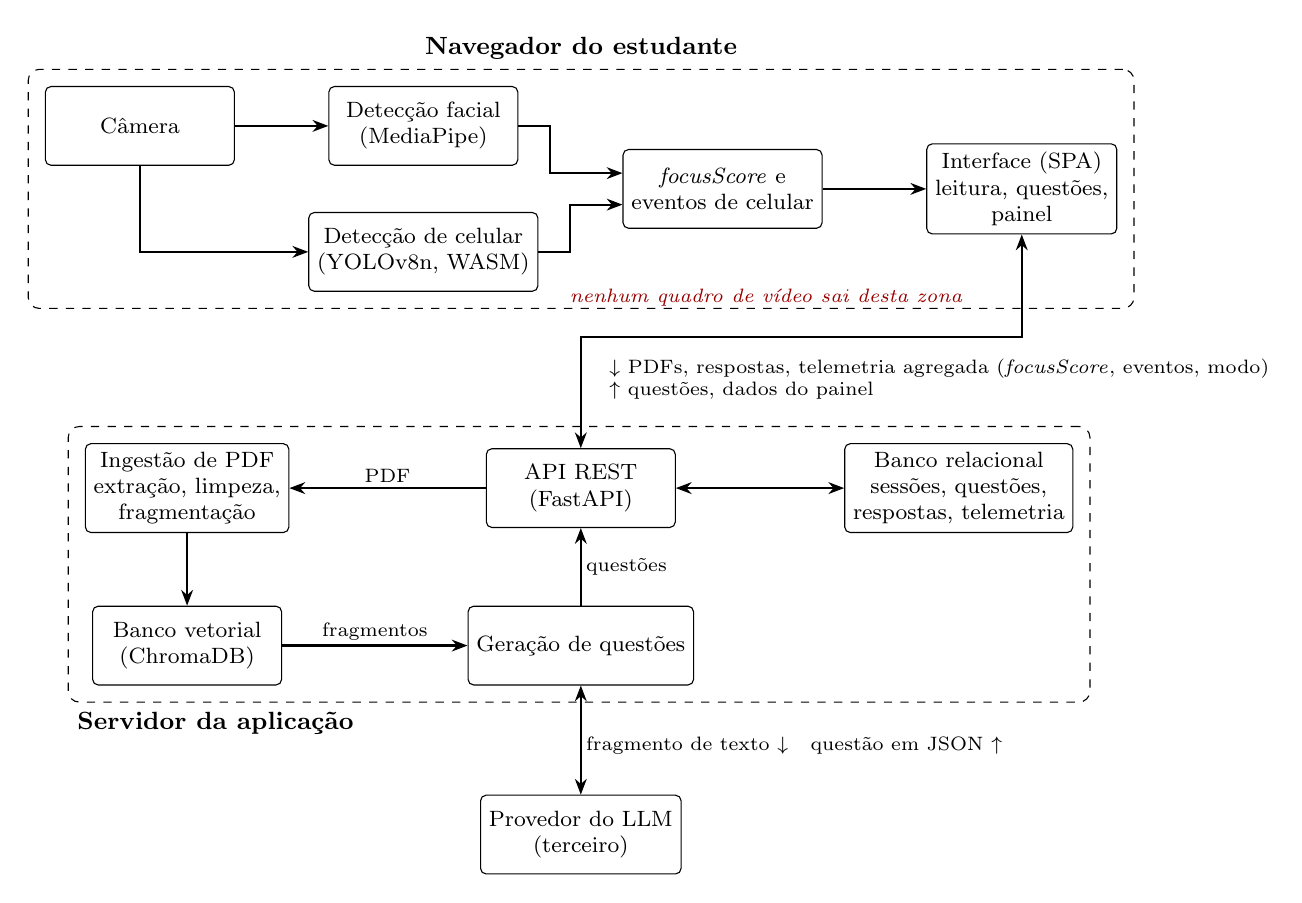
\begin{tikzpicture}[
  font=\footnotesize,
  caixa/.style={draw, rounded corners=2pt, align=center, minimum height=10mm, minimum width=24mm, inner sep=3pt, fill=white},
  zona/.style={draw, dashed, rounded corners=4pt, inner sep=6pt},
  seta/.style={-{Stealth[length=2mm]}, thick},
  rot/.style={font=\scriptsize, align=center, inner sep=1.5pt}
]
% ---- Navegador
\node[caixa] (cam) at (0,0) {Câmera};
\node[caixa] (fm) at (3.6,0) {Detecção facial\\(MediaPipe)};
\node[caixa] (yolo) at (3.6,-1.6) {Detecção de celular\\(YOLOv8n, WASM)};
\node[caixa] (ind) at (7.4,-0.8) {\fs e\\eventos de celular};
\node[caixa] (ui) at (11.2,-0.8) {Interface (SPA)\\leitura, questões,\\painel};
\draw[seta] (cam) -- (fm);
\draw[seta] (cam.south) |- (yolo.west);
\draw[seta] (fm.east) -- ++(0.4,0) |- ([yshift=2mm]ind.west);
\draw[seta] (yolo.east) -- ++(0.4,0) |- ([yshift=-2mm]ind.west);
\draw[seta] (ind) -- (ui);
\begin{scope}[on background layer]
\node[zona, fit=(cam)(fm)(yolo)(ind)(ui), label={[font=\small\bfseries]above:Navegador do estudante}] (nav) {};
\end{scope}
\node[rot, text=red!60!black, anchor=south west] at (5.4,-2.35) {\textit{nenhum quadro de vídeo sai desta zona}};

% ---- Servidor
\node[caixa] (ing) at (0.6,-4.6) {Ingestão de PDF\\extração, limpeza,\\fragmentação};
\node[caixa] (api) at (5.6,-4.6) {API REST\\(FastAPI)};
\node[caixa] (db) at (10.4,-4.6) {Banco relacional\\sessões, questões,\\respostas, telemetria};
\node[caixa] (vet) at (0.6,-6.6) {Banco vetorial\\(ChromaDB)};
\node[caixa] (ger) at (5.6,-6.6) {Geração de questões};
\draw[seta] (api) -- node[rot, above]{PDF} (ing);
\draw[seta] (ing) -- (vet);
\draw[seta] (vet) -- node[rot, above]{fragmentos} (ger);
\draw[seta] (ger) -- node[rot, right]{questões} (api);
\draw[seta, {Stealth[length=2mm]}-{Stealth[length=2mm]}] (api) -- (db);
\begin{scope}[on background layer]
\node[zona, fit=(ing)(api)(db)(vet)(ger), label={[font=\small\bfseries, anchor=north west]south west:Servidor da aplicação}] (srv) {};
\end{scope}

\node[caixa, minimum width=20mm] (llm) at (5.6,-9.0) {Provedor do LLM\\(terceiro)};
\draw[seta, {Stealth[length=2mm]}-{Stealth[length=2mm]}] (ger) -- node[rot, right, pos=0.55]{fragmento de texto $\downarrow$\quad questão em JSON $\uparrow$} (llm);

% ---- Tráfego cliente-servidor
\draw[seta, {Stealth[length=2mm]}-{Stealth[length=2mm]}] (ui.south) -- ++(0,-1.3) -| (api.north);
\node[rot, anchor=north west, align=left] at (5.9,-2.9) {$\downarrow$ PDFs, respostas, telemetria agregada (\fs, eventos, modo)\\$\uparrow$ questões, dados do painel};
\end{tikzpicture}
\caption{Arquitetura do \ferramenta. Toda a visão computacional ocorre na zona tracejada superior (navegador); o servidor recebe apenas os PDFs enviados pelo estudante, as respostas às questões e a telemetria agregada. O único dado que sai do servidor para um terceiro é o fragmento de texto enviado ao provedor do LLM. Fonte: elaborada pelo autor a partir do código do protótipo.}
\label{fig:arquitetura}
\end{figure}

A arquitetura segue uma regra simples: o que envolve a imagem do estudante fica no cliente; o que envolve o texto do material fica no servidor. O cliente é uma aplicação de página única (\estr{Single Page Application}, SPA) em Angular, que executa os dois modelos de visão computacional. O servidor, em Python com FastAPI, recebe os PDFs, mantém o banco vetorial e o banco relacional e orquestra as chamadas ao modelo de linguagem. A escolha do FastAPI se deve ao tratamento nativo de entrada e saída assíncrona e à validação declarativa dos dados recebidos, úteis para orquestrar chamadas a um serviço externo de latência variável e para garantir que a telemetria contenha apenas os campos esperados.

\section{\label{sec:mod1}Módulo 1: materiais e geração de questões}

\subsection{Ingestão do material}

O estudante cria uma disciplina e envia PDFs a ela (Figura~\ref{fig:materiais}). Cada PDF percorre quatro etapas. Primeiro, o texto é extraído página a página. Em seguida, uma etapa de limpeza remove hifenizações de fim de linha, junta linhas quebradas no meio de frases, normaliza marcadores de lista e descarta linhas repetidas, comuns em cabeçalhos e rodapés de apresentações. Depois, o texto limpo é fragmentado por um divisor recursivo que respeita, sempre que possível, quebras de parágrafo e de frase, com tamanho-alvo de 900 caracteres e sobreposição de 120 caracteres entre fragmentos consecutivos; fragmentos com menos de 80 caracteres são descartados. Por fim, os fragmentos são indexados no ChromaDB, em uma coleção por PDF.

\begin{figure}[htbp]
\centering
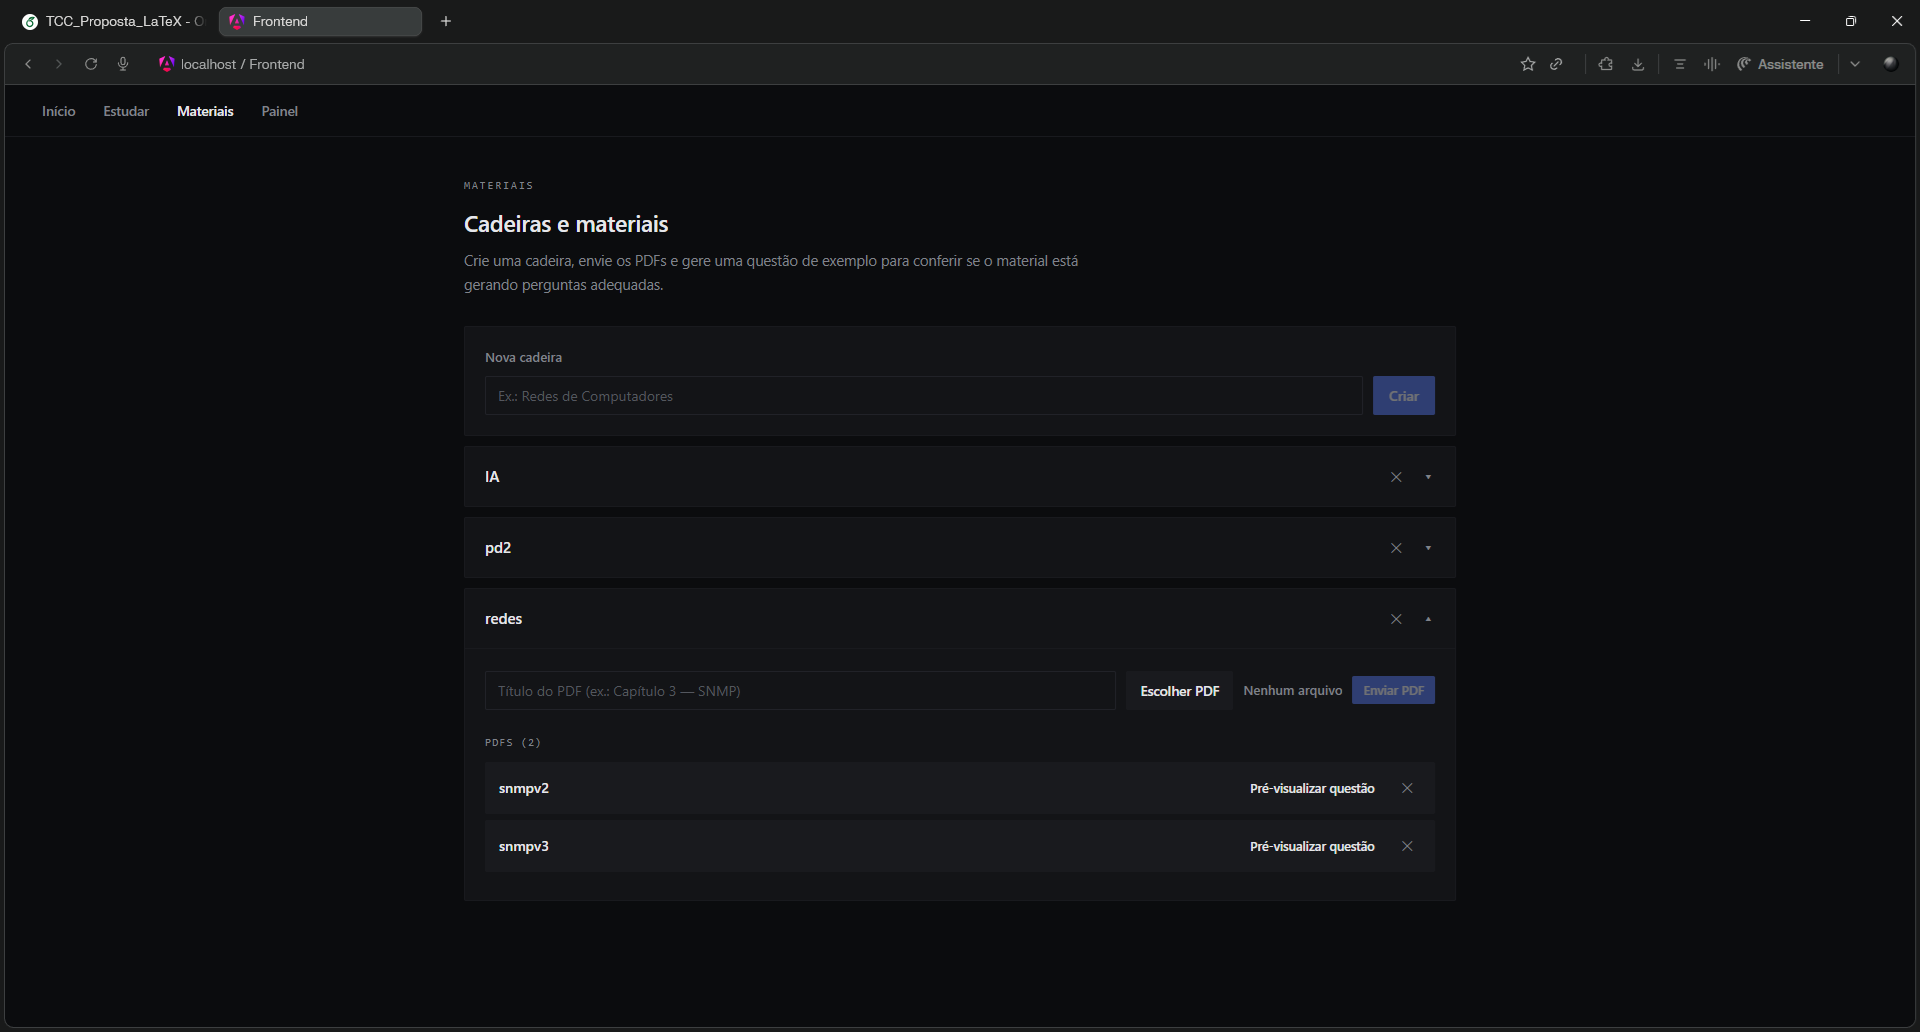
\includegraphics[width=0.85\textwidth]{materiais.png}
\caption[Tela de materiais do \ferramenta]{Tela de materiais: o estudante cria disciplinas, envia PDFs e pode pré-visualizar uma questão gerada a partir de um fragmento sorteado, para conferir se o material foi bem extraído. Fonte: captura do protótipo feita pelo autor. \definir{refazer a captura em tema claro, recortada e em resolução 2x}}
\label{fig:materiais}
\end{figure}

A sobreposição evita que uma ideia dividida entre dois fragmentos fique incompleta em ambos. O tamanho de 900 caracteres, aproximadamente dois parágrafos, busca um equilíbrio: fragmentos curtos demais não contêm informação suficiente para uma pergunta de compreensão, e fragmentos longos demais tornam difícil verificar se a resposta está neles. A sensibilidade dos resultados a esse parâmetro é avaliada na QP1 (Seção~\ref{sec:met-qp1}).

\subsection{Seleção do fragmento-fonte}

Nem todo fragmento de um PDF serve de base para uma pergunta: sumários, tabelas, listas de siglas e trechos de código produzem questões ruins. Antes da geração, cada fragmento passa por um filtro de utilidade que exige pelo menos 15 palavras e menos de 40\% delas em caixa alta, o que elimina a maior parte dos títulos e siglários. Se o filtro eliminar todos os fragmentos, o sistema usa os fragmentos originais, para não deixar o estudante sem questões. Dentre os fragmentos úteis dos PDFs selecionados para a sessão, o sistema sorteia os que servirão de fonte.

\subsection{Geração ancorada no fragmento}

Cada questão é gerada a partir de um único fragmento, chamado aqui de fragmento-fonte. O modelo recebe o fragmento e a instrução de criar uma questão de múltipla escolha em português, com enunciado respondível apenas com o conteúdo do trecho, quatro alternativas plausíveis e exatamente uma correta, acompanhada de uma justificativa. A resposta deve ser um objeto JSON com campos fixos. O prompt completo está no Apêndice~\ref{ap:prompts}.

Três cuidados complementam a geração. O primeiro é a validação do formato: respostas que não contêm um JSON válido ou que trazem menos de duas alternativas são rejeitadas. O segundo é o embaralhamento das alternativas após a geração, com a posição da correta recalculada, porque modelos de linguagem tendem a posicionar a alternativa correta de forma não uniforme. O terceiro é a rastreabilidade: o fragmento-fonte é gravado junto com a questão, o que permite, na revisão dos erros e na avaliação, conferir em que trecho a questão se baseou. Para reduzir a espera, as questões de uma sessão são geradas em lotes de cinco, em uma única chamada ao modelo, e o lote seguinte é solicitado enquanto o estudante responde ao atual.

Rigorosamente, o \ferramenta implementa uma variante da geração aumentada por recuperação. No RAG clássico, uma consulta do usuário é convertida em vetor e os fragmentos mais próximos são recuperados para compor o contexto. No \ferramenta, não há consulta: a ``recuperação'' é a escolha do fragmento que será perguntado, e o banco vetorial também permite recuperar os fragmentos vizinhos, semanticamente próximos, como contexto adicional. A versão principal gera a partir do fragmento-fonte isolado; a inclusão dos vizinhos é avaliada como ablação na QP1, justamente para medir se o contexto adicional melhora a questão ou a afasta do fragmento que deveria ancorá-la.

\section{\label{sec:mod2}Módulo 2: a sessão de estudo}

Ao iniciar uma sessão, o estudante escolhe os PDFs e uma de três atividades (Figura~\ref{fig:selecao}): responder a um questionário gerado do material; ler um material de estudo que o modelo produz a partir dos PDFs, adaptado ao nível, ao objetivo e ao tempo que o estudante declara; ou revisar as questões que errou em sessões anteriores. No questionário, cada resposta recebe \estr{feedback} imediato, com a indicação da alternativa correta e a justificativa (Figura~\ref{fig:quiz}), em linha com as condições de eficácia do \estr{feedback} discutidas na Seção~\ref{sec:perguntas}. O material de estudo gerado é um recurso de apoio e não é objeto da avaliação deste trabalho.

\begin{figure}[htbp]
\centering
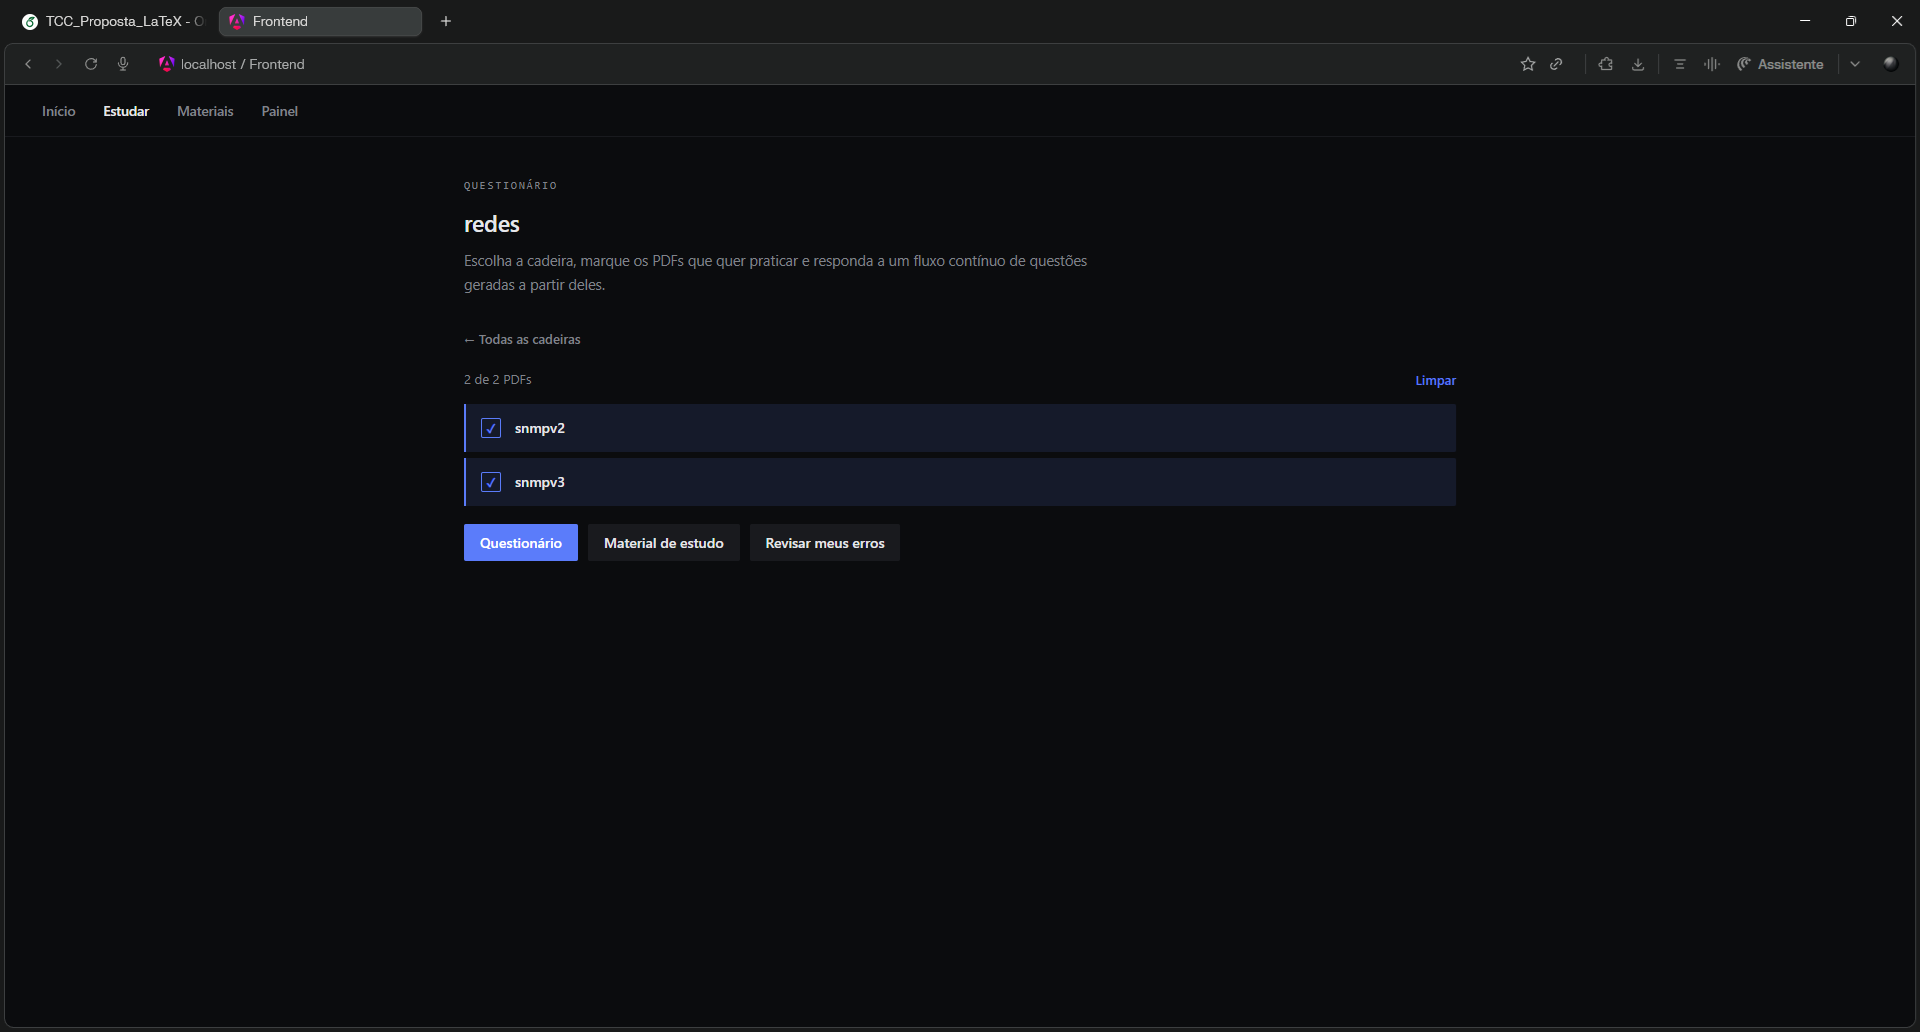
\includegraphics[width=0.85\textwidth]{selecao.png}
\caption{Início da sessão: seleção dos PDFs da disciplina e escolha entre questionário, material de estudo ou revisão dos erros. Fonte: captura do protótipo feita pelo autor.}
\label{fig:selecao}
\end{figure}

\begin{figure}[htbp]
\centering
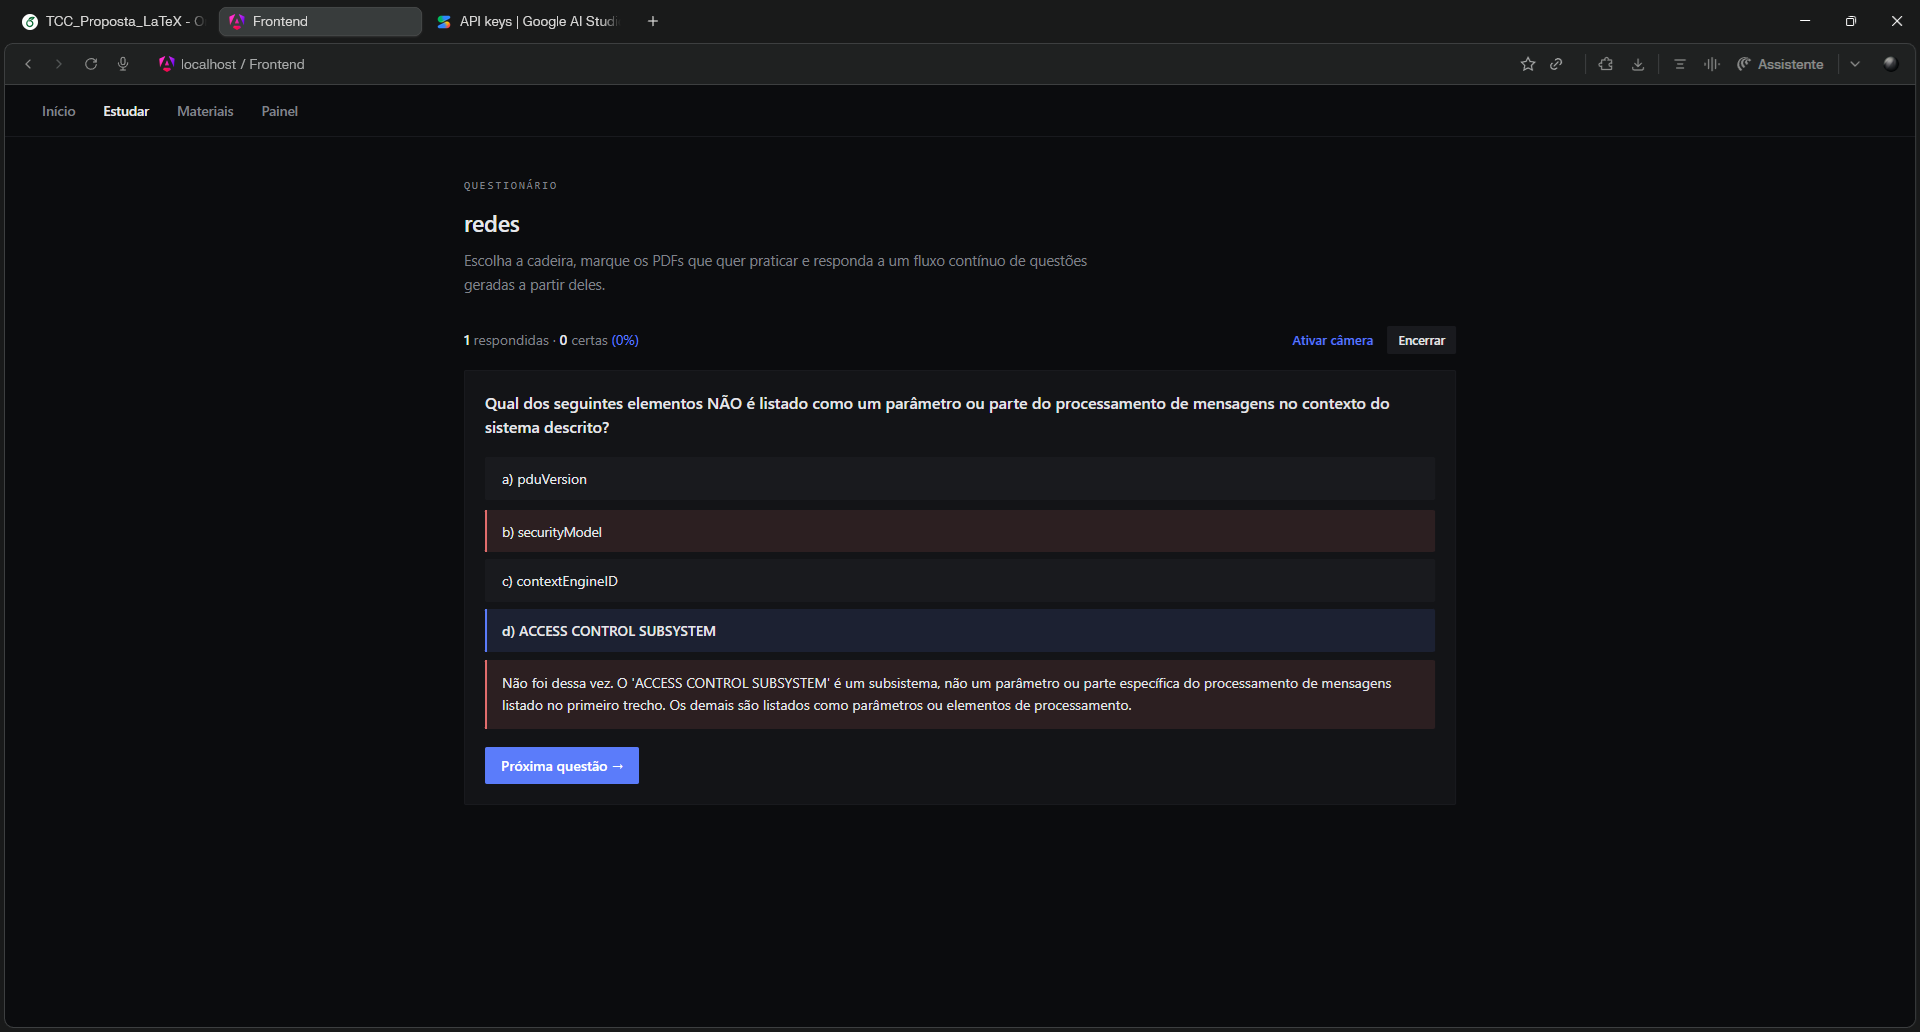
\includegraphics[width=0.85\textwidth]{quiz-feedback.png}
\caption{Questão gerada a partir de um fragmento do material, com \estr{feedback} imediato após a resposta: a alternativa correta é destacada e a justificativa é exibida. Fonte: captura do protótipo feita pelo autor.}
\label{fig:quiz}
\end{figure}

Com o consentimento do estudante, a câmera é ativada e dois processos passam a rodar no navegador: a estimativa do engajamento visual e a detecção de celular.

\subsection{\label{sec:focusscore}Engajamento visual: definição do \fs}

A cada quadro processado, o MediaPipe estima os pontos faciais a partir de um vídeo de 320$\times$240 \estr{pixels}. Três grandezas são calculadas sobre esses pontos.

A primeira é a EAR média dos dois olhos. Para cada olho, com os seis pontos $p_1,\dots,p_6$ dispostos ao seu redor ($p_1$ e $p_4$ nos cantos, $p_2,p_3$ na pálpebra superior e $p_6,p_5$ na inferior),
\begin{equation}
\mathrm{EAR} = \frac{\lVert p_2 - p_6\rVert + \lVert p_3 - p_5\rVert}{2\,\lVert p_1 - p_4\rVert}.
\label{eq:ear}
\end{equation}

A segunda e a terceira são aproximações da direção da cabeça, obtidas por razões entre coordenadas normalizadas dos pontos. A rotação horizontal (\estr{yaw}) é aproximada pela posição horizontal da ponta do nariz entre os dois contornos laterais do rosto, $y_{\mathrm{aw}} = (x_{\mathrm{nariz}} - x_{\mathrm{esq}})/(x_{\mathrm{dir}} - x_{\mathrm{esq}})$, que vale cerca de $0{,}5$ com o rosto de frente. A inclinação vertical (\estr{pitch}) é aproximada pela posição vertical da ponta do nariz entre a linha dos olhos e o queixo, $p_{\mathrm{itch}} = (y_{\mathrm{nariz}} - y_{\mathrm{olhos}})/(y_{\mathrm{queixo}} - y_{\mathrm{olhos}})$. Essas razões não são ângulos, mas variam de forma monotônica com eles e dispensam a estimativa de pose tridimensional.

Como os valores dessas grandezas variam entre pessoas, câmeras e posições, os primeiros cinco segundos da sessão são uma calibração, durante a qual o estudante olha para a tela. Ao final, o sistema guarda as medianas $\tilde{e}$, $\tilde{y}$ e $\tilde{p}$ da EAR, do \estr{yaw} e do \estr{pitch}, e define o limiar de olho aberto como $\theta = 0{,}72\,\tilde{e}$. O fator de $0{,}72$ foi ajustado em testes internos do autor e é objeto da análise de sensibilidade da QP3.

Após a calibração, cada quadro $i$ recebe um estado bruto $r_i \in \{0,1\}$, igual a 1 quando as três condições são satisfeitas simultaneamente:
\begin{equation}
r_i = \mathbb{1}\big[\text{rosto detectado}\big]\cdot
\mathbb{1}\big[\lvert y_{\mathrm{aw},i} - \tilde{y}\rvert < \tau_y \;\wedge\; \lvert p_{\mathrm{itch},i} - \tilde{p}\rvert < \tau_p\big]\cdot
\mathbb{1}\big[\mathrm{EAR}_i > \theta\big],
\label{eq:estado}
\end{equation}
com tolerâncias $\tau_y = 0{,}13$ e $\tau_p = 0{,}10$.

Um estado bruto igual a zero não significa necessariamente distração: piscar, olhar rapidamente para o teclado ou ajustar a postura produzem zeros de curta duração. Por isso, o sistema aplica um período de tolerância $g$: se o quadro $i$ pertence a uma sequência de estados brutos nulos iniciada no instante $t_d$, seu estado final é
\begin{equation}
s_i = \begin{cases} 1, & \text{se } r_i = 1 \text{ ou } t_i - t_d < g,\\ 0, & \text{caso contrário,}\end{cases}
\label{eq:tolerancia}
\end{equation}
com $g = 2{,}5$ s. O \fs no instante $t$ é, então, a porcentagem de quadros com estado final positivo em uma janela deslizante $W(t)$ de duração $\Delta = 8$ s:
\begin{equation}
\mathit{focusScore}(t) = 100 \cdot \frac{\sum_{i \in W(t)} s_i}{\lvert W(t)\rvert},
\qquad W(t) = \{\, i : t - t_i \le \Delta \,\}.
\label{eq:focusscore}
\end{equation}

A definição torna explícito o que o indicador mede: a fração recente do tempo em que o rosto esteve presente, voltado para a tela e com os olhos abertos, desconsiderando interrupções mais curtas que $g$. A Figura~\ref{fig:foco-estados} mostra o comportamento esperado em dois estados.

\begin{figure}[htbp]
\centering
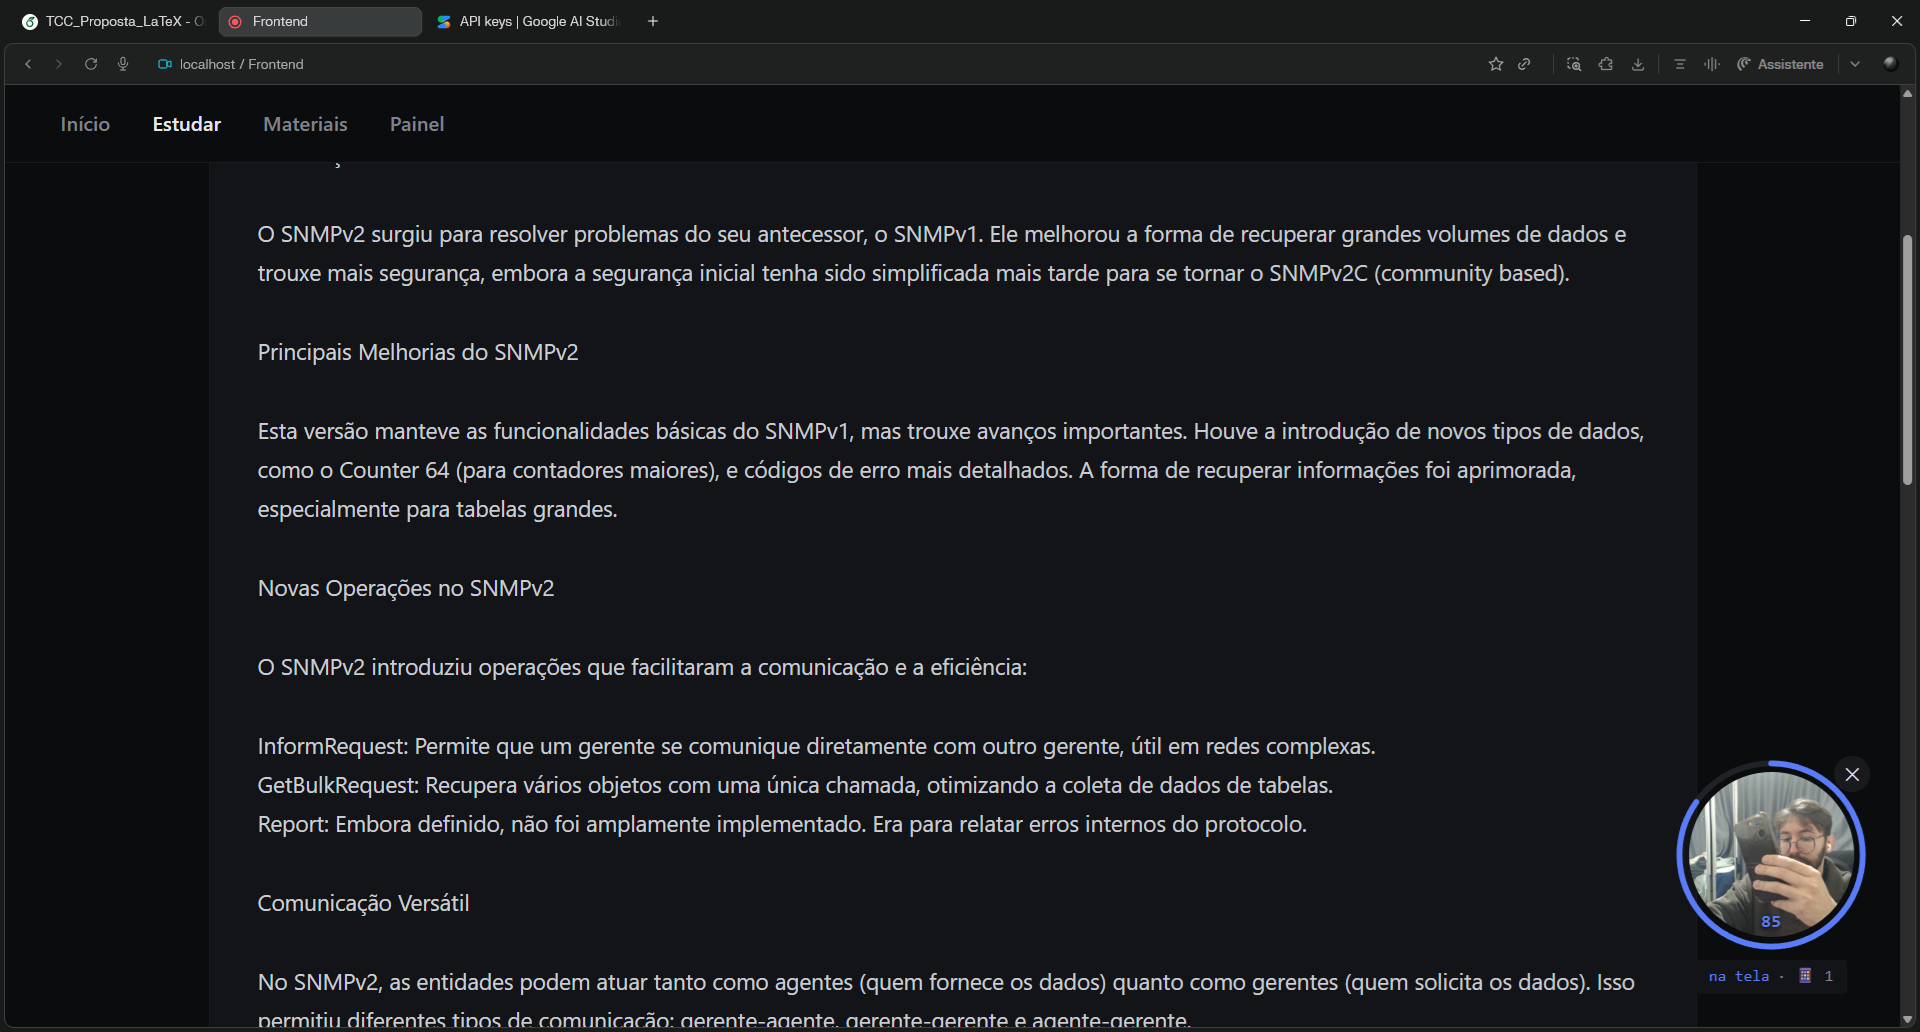
\includegraphics[width=0.48\textwidth]{foco-natela.png}\hfill
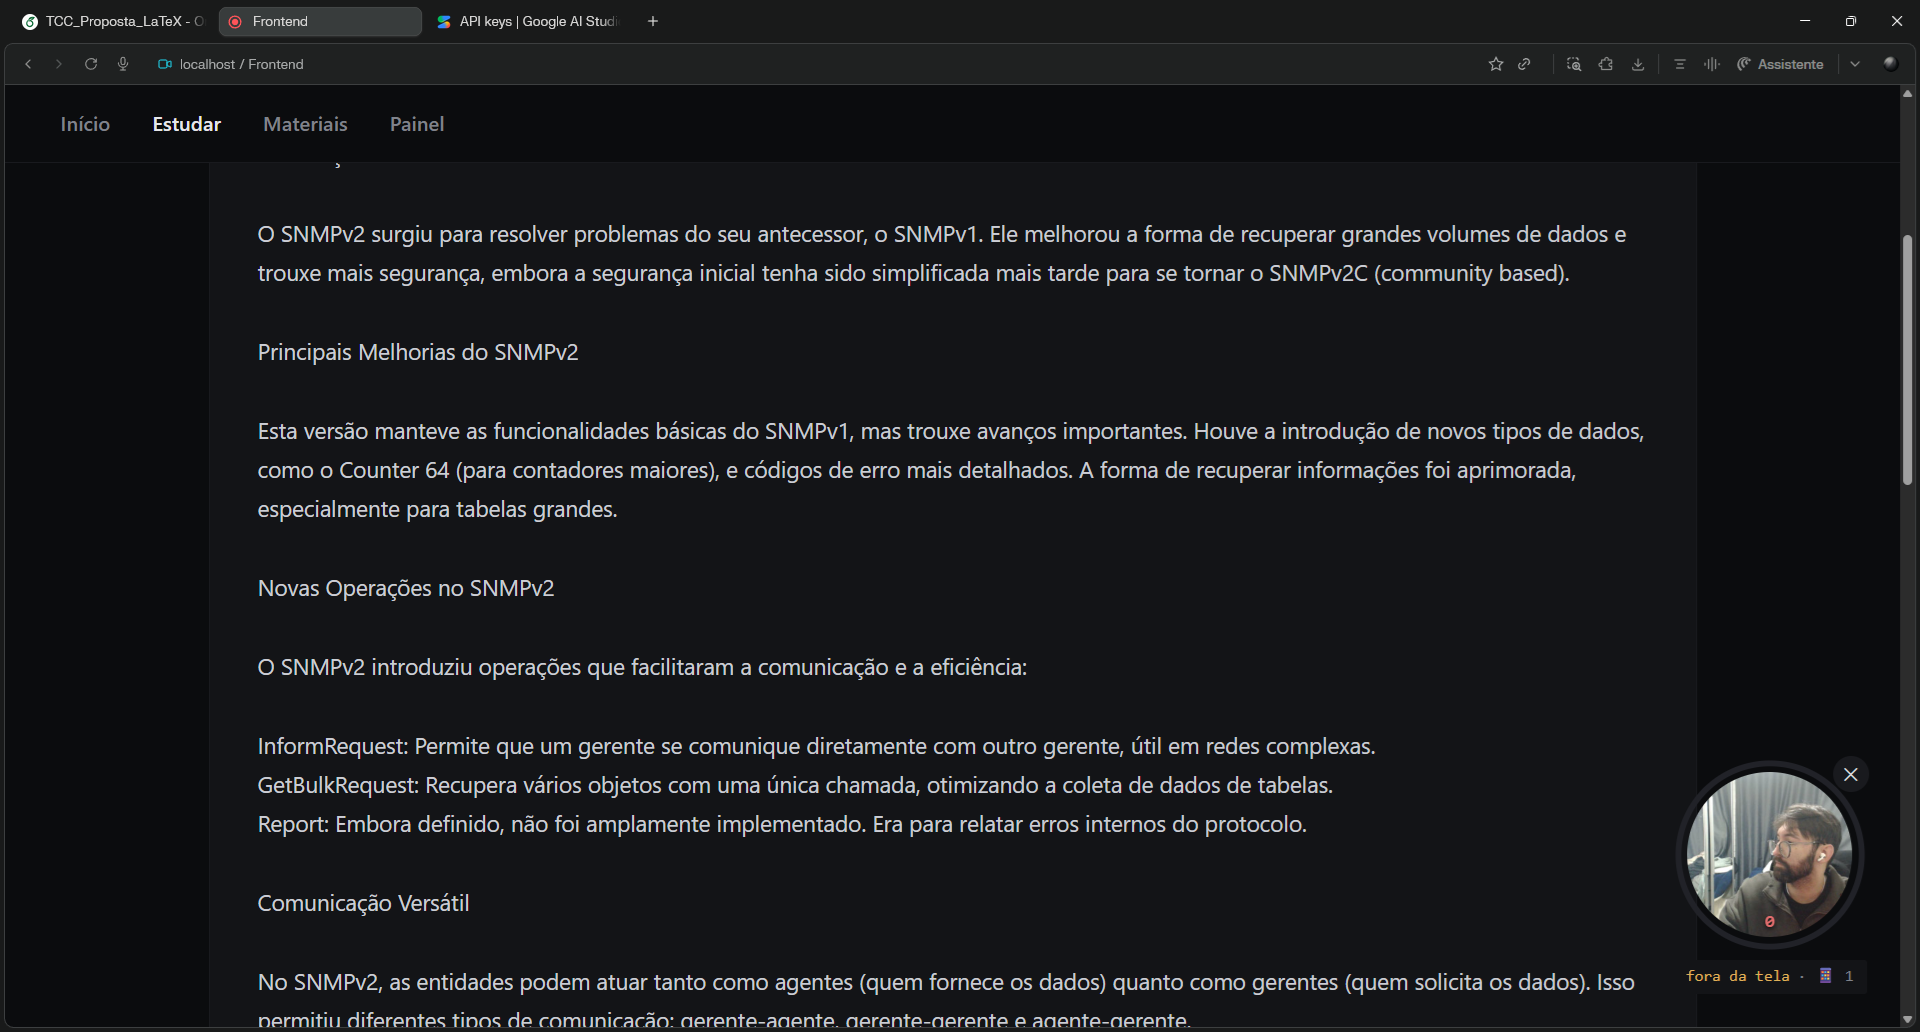
\includegraphics[width=0.48\textwidth]{foco-foratela.png}
\caption{Estados reconhecidos pelo monitoramento. À esquerda, rosto voltado para a tela, com um celular detectado no campo da câmera; à direita, olhar desviado da tela, com queda do \fs. Fonte: capturas do protótipo feitas pelo autor, com a própria imagem.}
\label{fig:foco-estados}
\end{figure}

\subsection{\label{sec:celular}Eventos de celular}

Em paralelo, a cada 1,2 s, o quadro atual é redimensionado para 640$\times$640 \estr{pixels}, com as bordas preenchidas para preservar a proporção, e submetido ao YOLOv8-nano pelo ONNX Runtime Web, em WebAssembly (WASM) com uma única \estr{thread}. Da saída da rede, o sistema extrai a maior pontuação atribuída à classe ``celular'' do COCO entre todas as posições candidatas, $c_j$. A inferência $j$ é positiva se $c_j > 0{,}35$. Um evento de celular é contado quando $k = 2$ inferências positivas consecutivas ocorrem, e um novo evento só pode começar depois que uma inferência negativa encerra o anterior. Com o intervalo de 1,2 s, isso significa que um celular precisa permanecer visível por cerca de 2,4 s para ser contado, o que filtra aparições acidentais. O número de eventos por intervalo de tempo é o segundo indicador enviado ao servidor.

\subsection{\label{sec:degradacao}Degradação graciosa}

Os dois modelos têm custos muito diferentes. A detecção facial é leve; o YOLO, mesmo na variante \estr{nano}, processa uma imagem de 640$\times$640 \estr{pixels} em uma rede convolucional, e seu tempo de inferência em WASM depende fortemente do processador. Em vez de exigir um computador mínimo, o \ferramenta degrada de forma graciosa: se o detector de celular não inicializa, ou se sua latência de inferência excede o intervalo de agendamento de 1,2 s de forma sustentada, ele é desligado, e a sessão continua apenas com o \fs. Se a própria detecção facial não inicializa, a sessão continua sem câmera, apenas com as questões. O modo de cada sessão (completo, sem celular ou sem câmera) é registrado junto com a telemetria. Essa decisão transforma uma limitação de \estr{hardware} em um comportamento previsível e mensurável, que é o objeto da QP2.

\section{\label{sec:mod3}Módulo 3: o painel de automonitoramento}

O painel (Figura~\ref{fig:painel}) devolve ao estudante, por disciplina, o tempo estudado, o tempo com \fs elevado, o \fs médio, o número de eventos de celular, o número de sessões e respostas, a taxa de acertos, a evolução do \fs minuto a minuto e a taxa de acertos por PDF. Seu propósito é alimentar o monitoramento do ciclo de autorregulação: tornar visível ao estudante, depois da sessão, o que ele não percebe durante ela.

\begin{figure}[htbp]
\centering
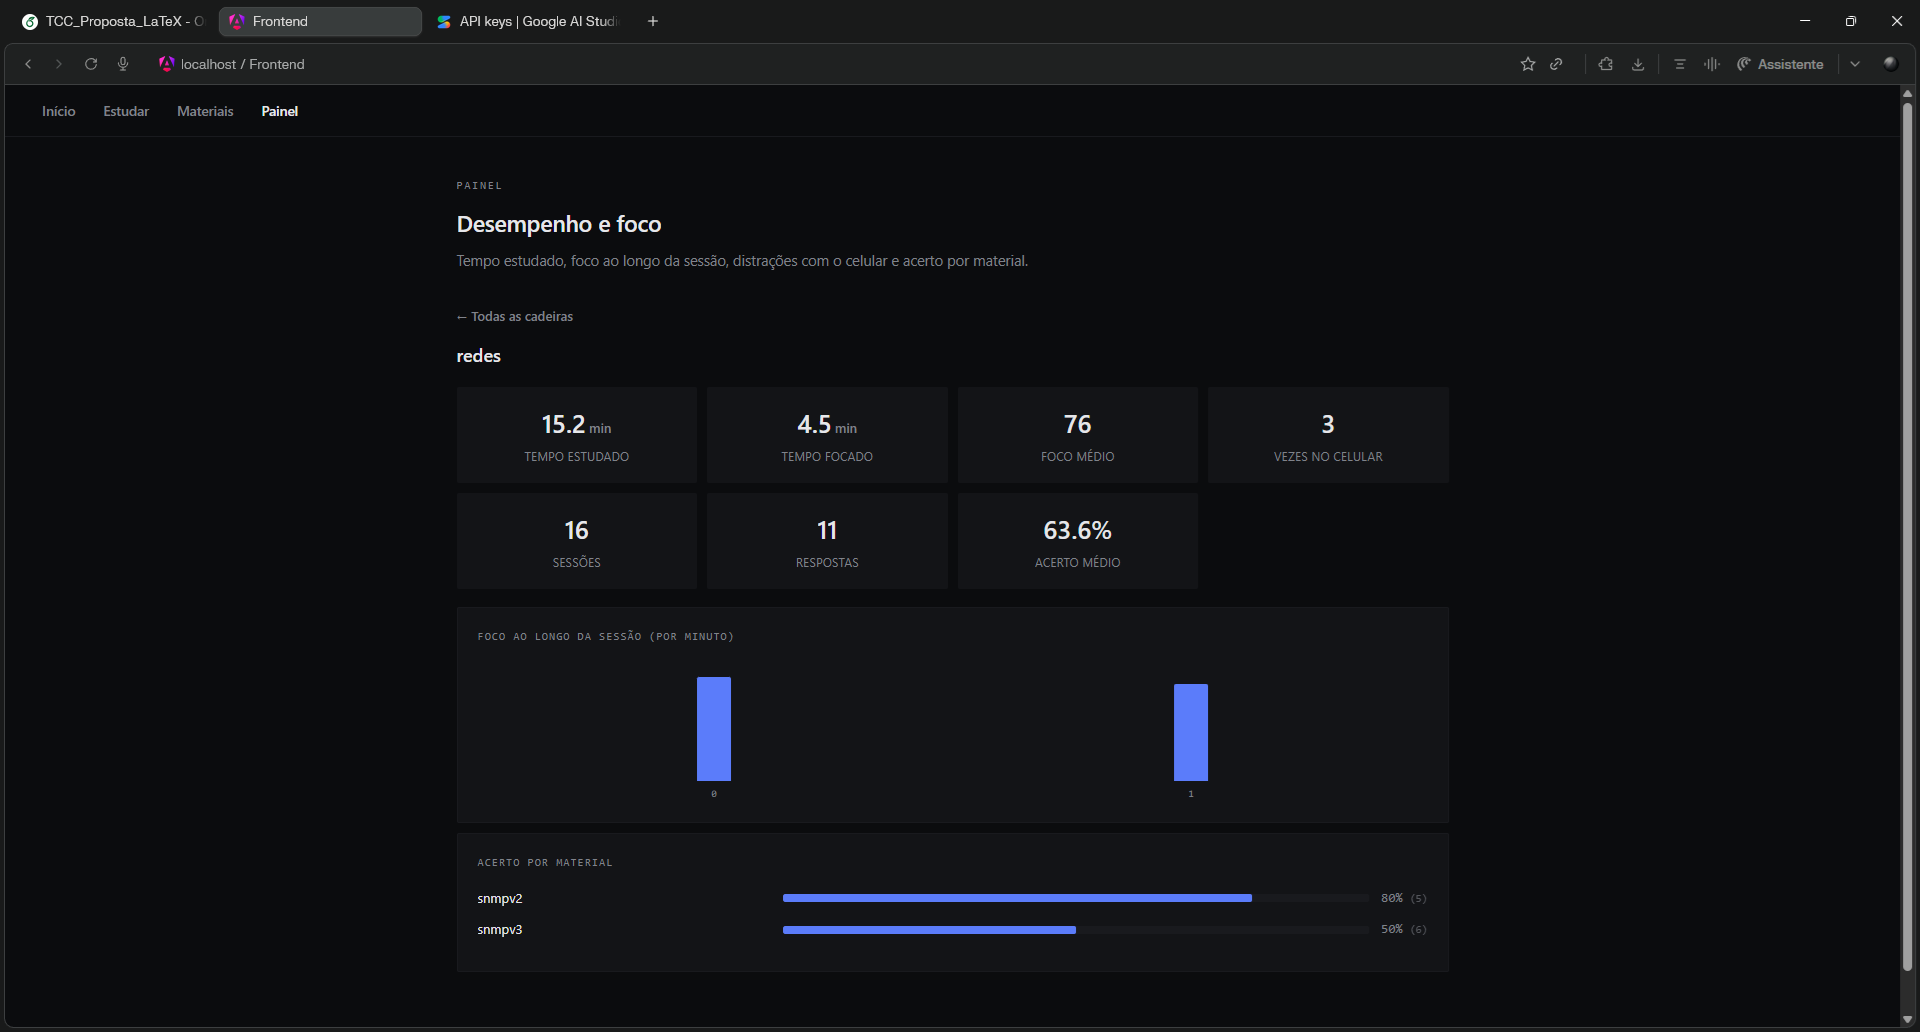
\includegraphics[width=0.85\textwidth]{painel.png}
\caption{Painel de automonitoramento de uma disciplina. Os valores exibidos provêm de sessões de teste do autor durante o desenvolvimento e ilustram apenas o \estr{layout}; não são resultados deste trabalho. Fonte: captura do protótipo feita pelo autor.}
\label{fig:painel}
\end{figure}

O painel cruza engajamento e desempenho, mas não afirma relação causal entre eles. Uma sessão com \fs baixo e muitos erros é um indício que o estudante pode interpretar, não um diagnóstico.

\section{\label{sec:fluxo}Fluxo de dados e privacidade}

O fluxo completo de uma sessão com câmera é o seguinte:
\begin{enumerate}
  \item O estudante envia o PDF; o servidor extrai, fragmenta e indexa o texto.
  \item O estudante inicia a sessão; o navegador carrega os modelos e calibra os limiares durante cinco segundos.
  \item A cada segundo, a interface atualiza o \fs exibido; a cada cinco segundos, grava uma amostra com o instante, o \fs, o número de novos eventos de celular e o modo da sessão; a cada quinze segundos, envia ao servidor o lote de amostras acumuladas.
  \item A cada questão, o fragmento-fonte correspondente foi enviado ao provedor do LLM no momento da geração, e a resposta do estudante é enviada ao servidor.
  \item O painel consulta o servidor, que agrega as amostras e as respostas.
\end{enumerate}

O fluxo tem duas fronteiras de privacidade distintas. A primeira, que envolve a imagem do estudante, é fechada por arquitetura: nenhum quadro de vídeo é serializado ou transmitido, e o servidor não tem sequer um \estr{endpoint} capaz de recebê-lo. A segunda, que envolve o texto do material, é aberta por necessidade: o fragmento-fonte precisa chegar ao modelo de linguagem, operado por terceiros. O estudante decide o que envia, mas deve ser informado de que o conteúdo dos PDFs sai do servidor da aplicação (Seção~\ref{sec:etica}). Há ainda um fluxo de dados de entrada menos evidente: os arquivos de execução e os pesos da detecção facial são baixados de redes de distribuição de conteúdo de terceiros, o que revela a esses serviços o endereço de rede do estudante, embora nenhuma imagem trafegue. A QP4 verifica a primeira fronteira e documenta os demais destinos contatados.

\section{\label{sec:parametros}Parâmetros da versão avaliada}

A Tabela~\ref{tab:parametros} reúne os parâmetros que definem o comportamento da versão avaliada. Os valores foram fixados antes da coleta e são os mesmos em todas as QPs, exceto nas análises de sensibilidade, que os variam de forma explícita.

\begin{table}[htbp]
\centering
\caption{Parâmetros da versão avaliada do \ferramenta. Fonte: código do protótipo \definir{versão/\estr{commit} congelado para a avaliação}.}
\label{tab:parametros}
\small
\begin{tabularx}{\textwidth}{>{\raggedright\arraybackslash}p{3.2cm} >{\raggedright\arraybackslash}X l}
\toprule
Componente & Parâmetro & Valor \\
\midrule
\multirow{3}{*}{Fragmentação} & Tamanho-alvo do fragmento & 900 caracteres \\
 & Sobreposição & 120 caracteres \\
 & Tamanho mínimo & 80 caracteres \\
\midrule
\multirow{2}{*}{Filtro de utilidade} & Mínimo de palavras & 15 \\
 & Máximo de palavras em caixa alta & 40\% \\
\midrule
\multirow{4}{*}{Geração} & Modelo de linguagem & \definir{modelo e versão} \\
 & Temperatura & 0,8 \\
 & Questões por chamada (lote) & 5 \\
 & \estr{Embeddings} & \definir{padrão do ChromaDB ou \estr{hashing}} \\
\midrule
\multirow{6}{*}{Engajamento visual} & Resolução de captura & 320$\times$240 \\
 & Duração da calibração & 5 s \\
 & Fator do limiar de EAR & 0,72 \\
 & Tolerâncias $\tau_y$, $\tau_p$ & 0,13; 0,10 \\
 & Período de tolerância $g$ & 2,5 s \\
 & Janela $\Delta$ & 8 s \\
\midrule
\multirow{4}{*}{Detecção de celular} & Entrada da rede & 640$\times$640 \\
 & Intervalo entre inferências & 1,2 s \\
 & Limiar de pontuação & 0,35 \\
 & Inferências consecutivas $k$ & 2 \\
\midrule
Telemetria & Amostragem / envio & 5 s / 15 s \\
\bottomrule
\end{tabularx}
\end{table}

Com o artefato definido, o próximo capítulo descreve como cada uma das promessas que ele assume será posta à prova.
% ===== fim de conteudo/cap3-ferramenta.tex =====

% ===== início de conteudo/cap4-metodologia.tex =====
% ===========================================================================
\chapter{\label{chap:metodo}Metodologia de Avaliação}

Este capítulo descreve como cada QP é respondida. A Seção~\ref{sec:abordagem} justifica a abordagem de avaliação técnica frente às alternativas. A Seção~\ref{sec:instrumentacao} lista a instrumentação acrescentada ao protótipo para a coleta. As Seções~\ref{sec:met-qp1} a~\ref{sec:met-qp4} apresentam, para cada QP, os dados, as condições comparadas, as métricas, os critérios definidos antes da coleta e as análises. A Seção~\ref{sec:met-usab} descreve a avaliação complementar de usabilidade e acessibilidade, e a Seção~\ref{sec:reprod} reúne o necessário para reproduzir o estudo. A Tabela~\ref{tab:sintese-metodo} resume o desenho.

\begin{table}[htbp]
\centering
\caption{Síntese do desenho de avaliação: para cada QP, os dados usados, as comparações, a métrica principal e o critério de viabilidade fixado antes da coleta. Fonte: elaborada pelo autor.}
\label{tab:sintese-metodo}
\small
\begin{tabularx}{\textwidth}{>{\raggedright\arraybackslash}p{1.6cm} >{\raggedright\arraybackslash}X >{\raggedright\arraybackslash}X >{\raggedright\arraybackslash}X >{\raggedright\arraybackslash}X}
\toprule
QP & Dados & Comparações & Métrica principal & Critério prévio \\
\midrule
QP1 Qualidade & 90 fragmentos de 3 materiais abertos & Proposta vs.\ linha de base sem fonte vs.\ linha de base por regras; ablação com vizinhos & Proporção de questões aceitáveis (IC 95\%) & $\ge 80\%$ aceitáveis na proposta \\
QP2 Viabilidade & Vídeo rotulado executado em 10 a 20 configurações de \estr{hardware} & Entre configurações e navegadores & FPS da detecção facial; latência p95 do YOLO & FPS mediano $\ge 5$; p95 $\le 1{,}2$ s \\
QP3 Validade & Vídeo roteirizado em 4 condições de gravação & Parâmetros padrão vs.\ variações (sensibilidade) & Acurácia balanceada por quadro; revocação de eventos & $\ge 0{,}80$ em ambas \\
QP4 Privacidade & Tráfego de rede de sessões automatizadas & Versão avaliada vs.\ controle positivo com vazamento & Requisições com conteúdo de imagem & Zero na versão avaliada; detecção no controle \\
\bottomrule
\end{tabularx}
\end{table}

\section{\label{sec:abordagem}Abordagem: avaliação técnica em \estr{Design Science Research}}

A \estr{Design Science Research} (DSR) produz conhecimento construindo um artefato que resolve um problema relevante e avaliando-o com rigor. O processo proposto por Peffers et al.\ \cite{PTR07} organiza essa atividade em etapas: identificar o problema, definir os objetivos da solução, projetar e desenvolver o artefato, demonstrá-lo, avaliá-lo e comunicar os resultados. Os Capítulos~\ref{chap:intro} a~\ref{chap:ferramenta} cobriram as quatro primeiras etapas; este capítulo trata da avaliação.

Hevner et al.\ admitem diferentes famílias de métodos de avaliação em DSR: observacionais, analíticos, experimentais, de teste e descritivos. A escolha deste trabalho recai sobre testes controlados do artefato, por três razões. A primeira é a correspondência com as QPs: as quatro dizem respeito a propriedades do artefato (qualidade do que ele gera, desempenho, validade de um indicador, fluxo de dados), e não ao comportamento de quem o usa. A segunda é a reprodutibilidade: um corpus fixo e um vídeo gravado permitem repetir cada medição, variar um parâmetro por vez e comparar versões, o que um estudo com participantes não permite. A terceira é a viabilidade: um estudo com participantes exigiria aprovação prévia do Comitê de Ética em Pesquisa, recrutamento e uma amostra maior do que a alcançável no calendário de um trabalho de conclusão para ter poder estatístico sobre efeitos de aprendizagem.

A alternativa descartada, um experimento com estudantes comparando sessões com e sem questões, responderia a uma pergunta diferente e mais ambiciosa, sobre o efeito da ferramenta na atenção ou no aprendizado. Essa pergunta só faz sentido depois que as propriedades básicas do artefato estiverem estabelecidas: não há por que medir o efeito de questões cuja qualidade é desconhecida, nem de um indicador cuja validade não foi verificada. A avaliação técnica é, portanto, pré-requisito do estudo com usuários, cujo desenho está no Apêndice~\ref{ap:usuarios}.

\section{\label{sec:instrumentacao}Instrumentação acrescentada ao protótipo}

A coleta exige quatro acréscimos ao protótipo descrito no Capítulo~\ref{chap:ferramenta}, todos sem efeito sobre o comportamento observado pelo estudante:

\begin{enumerate}
  \item \textbf{Registro de geração:} cada chamada ao LLM passa a registrar o modelo, a condição experimental, o fragmento-fonte, a latência, os \estr{tokens} de entrada e saída, se a resposta foi um JSON válido e, em caso de erro, o código de erro (incluindo limite de requisições).
  \item \textbf{Registro do modo da sessão:} o sucesso ou a falha da inicialização de cada modelo, o motivo da falha e a latência das primeiras inferências passam a ser gravados nos metadados da sessão, distinguindo os modos completo, sem celular e sem câmera (Seção~\ref{sec:degradacao}).
  \item \textbf{Página de \estr{benchmark}:} uma rota que reproduz um arquivo de vídeo em vez da câmera, executa os dois modelos por um tempo fixo e exibe, ao final, as medidas da QP2 em um arquivo que o próprio operador pode salvar.
  \item \textbf{Registro por quadro, apenas local:} no modo de \estr{benchmark}, as grandezas brutas de cada quadro (presença do rosto, EAR, \estr{yaw}, \estr{pitch}, pontuação $c_j$ do celular) são exportadas para um arquivo local, nunca enviado ao servidor. Esse registro permite recalcular o \fs com outros parâmetros sem reexecutar os modelos (Seção~\ref{sec:met-qp3}).
\end{enumerate}

\section{\label{sec:met-qp1}QP1: qualidade das questões geradas}

\subsection{Corpus}

O corpus é formado por três materiais didáticos de licença aberta, de áreas distintas, para evitar que os resultados reflitam um único estilo de texto: \definir{três capítulos de livros-texto abertos, com título, área, licença, número de páginas e formato (texto corrido ou apresentação de \estr{slides})}. Materiais abertos permitem publicar o corpus junto com o código. A inclusão de ao menos um material em formato de apresentação é deliberada: \estr{slides} produzem texto fragmentado, com listas e títulos soltos, que é o caso mais difícil para a extração e para a geração.

De cada material, são sorteados 30 fragmentos entre os que passam pelo filtro de utilidade (Seção~\ref{sec:mod1}), com semente fixa, totalizando 90 fragmentos. O tamanho da amostra foi escolhido pela precisão desejada: para uma proporção de questões aceitáveis próxima de 80\%, 90 questões por condição produzem um intervalo de confiança de 95\% pelo método de Wilson \cite{Wil27} com meia-largura de aproximadamente 8 pontos percentuais, suficiente para distinguir uma condição com 80\% de outra com 60\%, mas não diferenças pequenas. Essa limitação é assumida.

\subsection{Condições comparadas}

Para cada um dos 90 fragmentos, são geradas questões em quatro condições, o que produz um desenho pareado: a mesma unidade (o fragmento) é avaliada em todas as condições, e as diferenças entre condições não se confundem com diferenças entre fragmentos.

\begin{itemize}
  \item \textbf{P (proposta):} geração a partir do fragmento-fonte isolado, como na versão avaliada.
  \item \textbf{P+V (ablação com vizinhos):} geração a partir do fragmento-fonte acrescido dos dois fragmentos mais próximos no banco vetorial, identificados no prompt como contexto. Mede se o contexto adicional melhora a questão ou a desloca para fora do fragmento-fonte.
  \item \textbf{S (linha de base sem fonte):} o mesmo modelo, com o mesmo formato de saída, recebe apenas o título do material e o tema do fragmento, que é extraído por um procedimento automático \definir{procedimento de extração do tema, p.\ ex.\ o título de seção mais próximo}, mas não o texto do fragmento. Isola a contribuição da ancoragem: se S produzir questões tão boas quanto P, a ancoragem não estará agregando qualidade mensurável.
  \item \textbf{R (linha de base por regras):} o gerador extrativo, sem LLM, que o protótipo usa quando nenhum modelo está configurado. Ele escolhe termos salientes do fragmento, constrói o enunciado a partir da frase que os contém e usa outros termos do mesmo material como distratores. Representa o que se obtém sem modelo de linguagem.
\end{itemize}

A linha de base S é deliberadamente forte: ela usa o mesmo modelo, o mesmo prompt de formato e informação temática suficiente para gerar uma questão plausível sobre o assunto. A comparação justa não é entre um LLM e nada, mas entre gerar a partir do material e gerar a partir do conhecimento prévio do modelo sobre o mesmo tema.

\subsection{Inspeção humana}

As 360 questões (90 fragmentos $\times$ 4 condições) são avaliadas por dois avaliadores com domínio dos materiais, o autor e o orientador, com uma rubrica definida antes da geração e baseada nas diretrizes de redação de itens de Haladyna et al.\ (Seção~\ref{sec:geracao}):

\begin{itemize}
  \item \textbf{C1, ancoragem:} a alternativa correta é sustentada pelo fragmento-fonte? (sim / parcialmente / não)
  \item \textbf{C2, correção:} a alternativa indicada como correta está correta, e é a única correta? (sim / não)
  \item \textbf{C3, distratores:} quantos dos três distratores são plausíveis para quem não domina o conteúdo? (0 a 3)
  \item \textbf{C4, clareza:} o enunciado é inequívoco e gramaticalmente correto? (sim / não)
  \item \textbf{C5, nível cognitivo:} em qual nível da taxonomia revisada de Bloom \cite{AK01} a questão se situa? (lembrar / compreender / aplicar ou superior)
\end{itemize}

Uma questão é considerada \textbf{aceitável} quando C1 = sim, C2 = sim, C4 = sim e C3 $\ge 2$. A definição é conjuntiva porque uma questão falha, para o estudante, se falhar em qualquer desses aspectos: um gabarito errado ensina o erro, e uma questão não ancorada cobra o que o material não contém. C5 é descritivo e não entra no critério.

Para evitar que o conhecimento da condição influencie o julgamento, as questões são apresentadas aos avaliadores em ordem aleatória, sem identificação da condição, cada uma acompanhada apenas do seu fragmento-fonte. Na condição S, que não usou o fragmento, a ancoragem é avaliada contra o fragmento sorteado, o que é justamente o que se quer medir. Cada avaliador julga todas as questões de forma independente. A concordância é medida pelo coeficiente kappa de Cohen \cite{Coh60}, calculado antes de qualquer discussão e interpretado pelas faixas usuais de concordância (fraca, moderada, substancial, quase perfeita). As divergências são então discutidas até o consenso, e as análises usam as classificações de consenso.

\subsection{Métricas automáticas}

Além da inspeção, métricas automáticas são calculadas sobre todas as questões. Elas têm duas funções: detectar defeitos que a inspeção individual não revela, como vieses que só aparecem no agregado, e verificar se parte da inspeção pode ser automatizada em uso real, onde não há revisão humana.

\begin{itemize}
  \item \textbf{Ancoragem lexical:} proporção dos termos de conteúdo (excluídas palavras funcionais) da alternativa correta que aparecem no fragmento-fonte. É uma aproximação grosseira, que não reconhece paráfrases.
  \item \textbf{Juiz automático:} um LLM de família diferente da do gerador, para mitigar o viés de autopreferência discutido na Seção~\ref{sec:geracao}, recebe o fragmento, a questão e a pergunta C1 da rubrica. As alternativas são apresentadas em duas ordens, e a classificação só é aceita se for igual nas duas, para mitigar o viés de posição. \definir{modelo usado como juiz}
  \item \textbf{Falhas de formato:} proporção de chamadas com JSON inválido, com menos de quatro alternativas ou encerradas por erro, incluindo limite de requisições.
  \item \textbf{Viés de posição:} distribuição da posição da alternativa correta, que deve ser uniforme após o embaralhamento; testada pelo qui-quadrado de aderência.
  \item \textbf{Viés de extensão:} proporção de questões em que a alternativa correta é estritamente a mais longa. Sem viés, o valor esperado é próximo de 25\%; valores muito maiores indicam uma pista que permite acertar sem conhecer o conteúdo.
  \item \textbf{Duplicatas:} pares de questões do mesmo material cujos enunciados têm similaridade de cosseno acima de 0,9 entre seus \estr{embeddings}.
  \item \textbf{Custo e latência:} latência por chamada e por lote, \estr{tokens} por questão e custo estimado pela tabela de preços do provedor na data da coleta.
\end{itemize}

\subsection{Análise}

Para cada condição, reporta-se a proporção de questões aceitáveis e de cada critério, com intervalo de confiança de 95\% de Wilson. As comparações de interesse são P contra S (efeito da ancoragem), P contra R (efeito do LLM) e P contra P+V (efeito do contexto adicional). Como os dados são pareados e binários, cada comparação usa o teste de McNemar \cite{McN47}, com correção de Holm para as três comparações, e reporta a diferença de proporções com intervalo de confiança por \estr{bootstrap} pareado como medida de tamanho de efeito. A concordância entre o juiz automático e o consenso humano no critério C1 é reportada por kappa, assim como a concordância entre a ancoragem lexical, dicotomizada por um limiar escolhido no primeiro material e aplicado aos outros dois, e o consenso humano.

\subsection{Sensibilidade e variabilidade}

Duas análises verificam se as conclusões dependem de escolhas arbitrárias. Na primeira, um subconjunto de 30 fragmentos é refragmentado com tamanhos-alvo de 600 e 1.200 caracteres, e as questões da condição P são geradas e inspecionadas novamente. Na segunda, como a geração a temperatura 0,8 não é determinística, as questões da condição P de 30 fragmentos são geradas três vezes, e a variação da proporção de aceitáveis entre repetições estima a variabilidade atribuível ao sorteio do modelo. Os critérios métricos do teste principal são reaplicados sem alteração.

\section{\label{sec:met-qp2}QP2: viabilidade da visão computacional no navegador}

\subsection{Procedimento}

A QP2 mede o desempenho dos dois modelos em computadores reais sem que nenhuma pessoa seja filmada. Para isso, a página de \estr{benchmark} (Seção~\ref{sec:instrumentacao}) substitui a câmera por um vídeo pré-gravado: o mesmo vídeo roteirizado da QP3, reproduzido do disco. O uso de um vídeo fixo tem duas vantagens: a carga de trabalho é idêntica em todas as máquinas, e as medidas de desempenho não dependem da câmera ou do ambiente de cada operador.

Cada execução dura cinco minutos e segue os mesmos passos da sessão real: carregar os modelos, calibrar durante cinco segundos e processar o vídeo com os parâmetros da Tabela~\ref{tab:parametros}. Ao final, a página exibe as medidas e oferece um arquivo para o operador salvar e enviar.

\subsection{Amostra de configurações}

A amostra é de conveniência e busca variedade, não representatividade estatística: de 10 a 20 configurações, entendidas como a combinação de computador e navegador, incluindo as máquinas do autor, computadores de laboratório da universidade \definir{laboratórios e autorização de uso} e \estr{notebooks} de colegas que executem voluntariamente a página. Busca-se cobrir ao menos: processadores de entrada, intermediários e de alto desempenho; computadores com e sem placa de vídeo dedicada; e os navegadores Chrome, Edge e Firefox. Os dados coletados descrevem a máquina, não a pessoa: número de núcleos lógicos, memória informada pelo navegador, modelo do processador quando declarado, navegador e versão, disponibilidade de WebGL e de instruções vetoriais em WASM.

\subsection{Métricas e critérios}

\begin{itemize}
  \item \textbf{Inicialização:} sucesso ou falha de cada modelo e tempo até o primeiro resultado.
  \item \textbf{Detecção facial:} taxa de quadros processados por segundo (FPS), com mediana e percentil 5, e tempo de processamento por quadro, com mediana e percentil 95.
  \item \textbf{Detecção de celular:} latência por inferência, com mediana e percentil 95, e intervalo efetivo entre inferências.
  \item \textbf{Responsividade da interface:} número de tarefas longas da \estr{thread} principal, definidas pelo navegador como execuções acima de 50 ms, por minuto.
  \item \textbf{Memória:} uso de memória do \estr{heap} de JavaScript ao final da execução, quando o navegador o informa.
  \item \textbf{Modo resultante:} completo, sem celular ou sem câmera, segundo a regra da Seção~\ref{sec:degradacao}.
  \item \textbf{Tempo até a primeira questão:} medido no servidor, do pedido do primeiro lote à sua entrega, em sessões da QP1.
\end{itemize}

Os critérios de viabilidade foram derivados dos próprios parâmetros do sistema e de limites clássicos de tempo de resposta, e fixados antes da coleta. A detecção facial é considerada operável com FPS mediano de pelo menos 5, porque, com o período de tolerância $g = 2{,}5$ s, essa taxa garante ao menos 12 quadros por período, e a janela de 8 s passa a conter ao menos 40 quadros, o que dá ao \fs resolução melhor que 2,5 pontos. O percentil 95 do tempo por quadro deve ficar abaixo de 100 ms, limite abaixo do qual a resposta de um sistema é percebida como instantânea \cite{Nie93}, para que o processamento não prejudique a leitura. O detector de celular é considerado viável quando o percentil 95 de sua latência não excede o intervalo de agendamento de 1,2 s; acima disso, o intervalo efetivo cresce, e a duração mínima de um evento aumenta com ele. O tempo até a primeira questão deve ficar abaixo de 10 s, limite para manter a atenção do usuário na tarefa.

\subsection{Análise}

Os resultados são reportados por configuração, em tabela, e sintetizados em gráficos de dispersão que relacionam o número de núcleos lógicos ao FPS mediano da detecção facial e à latência mediana do YOLO. A proporção de configurações em que cada modelo é viável e a proporção em que o modo degradado é acionado são reportadas com IC de 95\% de Wilson. Com amostras dessa ordem, os intervalos serão largos; por isso, a análise privilegia a descrição de onde a viabilidade se rompe (quais combinações de \estr{hardware} e navegador) em vez de uma estimativa populacional.

\section{\label{sec:met-qp3}QP3: validade do indicador de engajamento}

\subsection{Roteiro e gravação}

A validade do \fs é verificada contra estados comportamentais conhecidos, representados pelo próprio autor diante da câmera, seguindo um roteiro. Uma página auxiliar exibe as instruções na tela e registra automaticamente o instante de início e de fim de cada segmento, o que produz os rótulos sem anotação manual. O roteiro tem oito segmentos, cada um com um estado esperado (Tabela~\ref{tab:roteiro}).

\begin{table}[htbp]
\centering
\caption{Roteiro do vídeo rotulado. ``Atento esperado'' é o estado que o \fs deveria refletir; ``Evento esperado'' indica se o detector de celular deveria registrar um evento. Fonte: elaborada pelo autor.}
\label{tab:roteiro}
\small
\begin{tabularx}{\textwidth}{c >{\raggedright\arraybackslash}X c c c}
\toprule
Seg. & Comportamento & Duração & Atento esperado & Evento esperado \\
\midrule
S1 & Leitura na tela, postura natural & 60 s & Sim & Não \\
S2 & Leitura com piscadas e olhadas breves ($<2$ s) ao teclado & 45 s & Sim & Não \\
S3 & Olhar lateral sustentado, como para outra tela & 20 s & Não & Não \\
S4 & Olhar para baixo sustentado, como para um caderno & 20 s & Não & Não \\
S5 & Olhos fechados & 15 s & Não & Não \\
S6 & Rosto fora do campo da câmera & 15 s & Não & Não \\
S7 & Uso do celular na mão, olhando para ele & 30 s & Não & Sim \\
S8 & Celular sobre a mesa, visível, olhar na tela & 30 s & Sim & Sim \\
\bottomrule
\end{tabularx}
\end{table}

Dois segmentos merecem justificativa. O S2 testa o período de tolerância: piscadas e olhadas curtas não devem derrubar o indicador. O S8 separa a presença do celular do seu uso: como o detector reconhece o objeto, e não o comportamento, espera-se que ele conte um evento mesmo com o estudante atento. O resultado de S8 não mede um erro do detector, mas delimita o que o indicador significa.

O roteiro é gravado em quatro condições, combinando iluminação adequada ou fraca e uso ou não de óculos, fatores que afetam a detecção dos pontos dos olhos. Cada gravação tem cerca de quatro minutos. Os segmentos são separados por intervalos de transição, e os quadros situados até 1 s antes ou depois de cada fronteira são excluídos das métricas, para que imprecisões na mudança de comportamento não sejam contadas como erro do indicador.

\subsection{Métricas e critérios}

O estado final $s_i$ de cada quadro (Equação~\ref{eq:tolerancia}) é comparado ao estado esperado do segmento. Como os segmentos desatentos são mais curtos que os atentos, a métrica principal é a acurácia balanceada, média entre a sensibilidade (proporção de quadros desatentos corretamente identificados) e a especificidade (proporção de quadros atentos corretamente identificados), que não é inflada pelo desbalanceamento. Reportam-se também a matriz de confusão por segmento e o atraso de detecção, definido como o tempo entre o início de um segmento desatento e o primeiro instante em que o \fs cai abaixo de 50.

Para o detector de celular, as métricas são a revocação por evento, proporção dos segmentos S7 e S8 em que ao menos um evento foi contado, e a taxa de falsos eventos, número de eventos contados nos segmentos S1 a S6 por dez minutos de vídeo.

Os critérios fixados antes da coleta são acurácia balanceada de pelo menos 0,80 com os parâmetros padrão, revocação de eventos de pelo menos 0,80 e no máximo um falso evento por dez minutos. São critérios de projeto, e não padrões da literatura: correspondem a um indicador que acerta, em média, quatro de cada cinco quadros de cada classe e que não interrompe o estudante com alarmes frequentes.

\subsection{Sensibilidade aos parâmetros}

Como o registro por quadro guarda as grandezas brutas, o \fs pode ser recalculado para qualquer combinação de parâmetros sem reprocessar o vídeo. A análise varia um parâmetro por vez, mantendo os demais no padrão:

\begin{itemize}
  \item limiar de EAR: calibrado por sessão (padrão) contra um limiar fixo, igual à média dos limiares calibrados das quatro gravações;
  \item fator do limiar de EAR: 0,60; 0,72; 0,85;
  \item tolerâncias de direção da cabeça: metade, padrão e uma vez e meia os valores de $\tau_y$ e $\tau_p$;
  \item período de tolerância $g$: 0; 1,5; 2,5; 4 s;
  \item janela $\Delta$: 4; 8; 16 s;
  \item limiar de pontuação do celular: 0,25; 0,35; 0,50;
  \item inferências consecutivas $k$: 1, 2, 3.
\end{itemize}

A comparação entre limiar calibrado e fixo é a ablação mais importante, porque testa uma decisão de projeto defendida na Seção~\ref{sec:engajamento}: a de que a variação individual da EAR exige calibração.

\section{\label{sec:met-qp4}QP4: verificação automatizada da privacidade}

\subsection{Teste de tráfego}

Um teste automatizado, escrito com a biblioteca Playwright, executa uma sessão completa em um navegador Chromium cuja câmera é substituída pelo vídeo roteirizado: envia um PDF, inicia uma sessão com câmera, responde a dez questões, permanece cinco minutos na leitura e encerra a sessão. Durante toda a execução, o teste intercepta e registra todas as requisições de rede, com destino, método, tamanho e corpo.

Sobre esse registro, o teste verifica três propriedades. Primeiro, que toda requisição dirigida ao servidor da aplicação corresponda a um \estr{endpoint} esperado e contenha apenas os campos previstos em seu esquema. Segundo, que nenhum corpo de requisição, para qualquer destino, contenha assinaturas de imagem (cabeçalhos binários de JPEG, PNG ou WebP, ou o prefixo \texttt{data:image}) nem sequências em base64 com mais de 1 KB. Terceiro, que o tamanho das requisições de telemetria seja compatível com o esquema, da ordem de centenas de \estr{bytes} por lote. O teste também produz a lista de todos os domínios externos contatados, com a finalidade de cada um.

\subsection{Controle positivo}

Um teste que não encontra vazamento só é informativo se for capaz de encontrá-lo quando ele existe. Por isso, o mesmo teste é executado contra uma versão modificada do cliente que, deliberadamente, envia ao servidor um quadro da câmera codificado em JPEG a cada minuto. O critério da QP4 exige duas coisas: zero requisições com conteúdo de imagem na versão avaliada e detecção de todos os envios na versão com vazamento.

\subsection{Revisão estática}

Como complemento, o código do cliente é inspecionado em busca de todas as chamadas capazes de serializar imagens (\texttt{toDataURL}, \texttt{toBlob}, \texttt{getImageData}) e de todas as chamadas de rede, e cada ocorrência é justificada. O uso de \texttt{getImageData}, por exemplo, é esperado: é assim que o quadro é convertido no tensor de entrada do YOLO, dentro do navegador.

\section{\label{sec:met-usab}Avaliação complementar: usabilidade e acessibilidade}

Embora não seja objeto de uma QP, a interface é avaliada por dois métodos de inspeção, que não envolvem participantes na condição de sujeitos. O primeiro é a inspeção heurística com as dez heurísticas de Nielsen \cite{Nie94}, aplicada a três tarefas: enviar um material, realizar uma sessão de estudo com câmera e interpretar o painel. Cada problema encontrado é registrado com a heurística violada e uma severidade de 0 a 4. O número recomendado de avaliadores é de três a cinco; a composição do grupo é \definir{avaliadores da inspeção heurística e confirmação, com o orientador, de que a inspeção por colegas não exige submissão ao CEP}. O segundo método é a auditoria automática de acessibilidade das quatro telas principais com as ferramentas Lighthouse e axe-core, que verificam critérios das Diretrizes de Acessibilidade para Conteúdo Web (WCAG) 2.1 \cite{W3C18}, como contraste, rótulos de controles e navegação por teclado.

\section{\label{sec:reprod}Ambiente e reprodutibilidade}

O servidor executa em Python 3 com FastAPI, SQLAlchemy, pypdf, o divisor de texto do LangChain e ChromaDB; o cliente, em Angular 19, com MediaPipe Tasks Vision e ONNX Runtime Web \referencia{documentação ou artigo de referência do ONNX Runtime}. As versões exatas de todas as dependências são fixadas no repositório. \definir{sistema operacional, processador e memória da máquina que executa o servidor e a geração}.

Todos os sorteios usam sementes fixas registradas. O repositório público \definir{endereço do repositório} contém o código na versão avaliada, os três materiais do corpus, as questões geradas com suas classificações, os registros de geração, os arquivos das execuções de \estr{benchmark}, os registros por quadro das gravações e os \estr{scripts} de análise. As gravações de vídeo, por conterem a imagem do autor, não são publicadas; os registros por quadro, que contêm apenas grandezas numéricas, permitem reproduzir todas as análises da QP3.

O próximo capítulo apresenta os resultados na mesma ordem das QPs.
% ===== fim de conteudo/cap4-metodologia.tex =====

% ===== início de conteudo/cap5-resultados.tex =====
% ===========================================================================
\chapter{\label{chap:resultados}Resultados}

% Caixa para figuras ainda não produzidas
\newcommand{\figurapendente}[1]{%
  \fbox{\begin{minipage}[c][4.2cm][c]{0.9\textwidth}\centering\small
  \textcolor{red!70!black}{\textbf{[FIGURA PENDENTE]}}\\[2pt] #1\end{minipage}}}

Este capítulo reporta os resultados na ordem das QPs. Nas tabelas, a marca \rr\ indica uma célula a preencher com o resultado da coleta. Os resultados são apresentados sem interpretá-los além do necessário para lê-los; a interpretação é feita no Capítulo~\ref{chap:discussao}. Todos os números provêm da coleta descrita no Capítulo~\ref{chap:metodo}, e cada tabela e figura indica sua fonte. \resultado{período de coleta, versão (\estr{commit}) avaliada e eventuais desvios em relação ao protocolo, com justificativa}.

\section{QP1: qualidade das questões}

\subsection{Concordância entre avaliadores}

\resultado{kappa de Cohen entre os dois avaliadores, antes da discussão, para cada critério C1 a C5, com a interpretação pelas faixas usuais de concordância; número de divergências resolvidas por discussão}. Esse resultado precede os demais porque condiciona sua leitura: se a concordância for baixa em algum critério, as proporções desse critério devem ser tratadas com cautela.

\subsection{Proporção de questões aceitáveis}

A Tabela~\ref{tab:qp1-principal} apresenta, para cada condição, a proporção de questões que atendem a cada critério e ao critério conjunto de aceitabilidade.

\begin{table}[htbp]
\centering
\caption{Qualidade das questões por condição, segundo o consenso dos avaliadores ($n = 90$ questões por condição). Valores em porcentagem, com IC de 95\% de Wilson entre colchetes. C1 conta apenas ``sim''; C3 conta questões com ao menos dois distratores plausíveis. Fonte: dados da coleta da QP1.}
\label{tab:qp1-principal}
\small
\begin{tabular}{lccccc}
\toprule
Condição & C1 Ancoragem & C2 Correção & C3 Distratores & C4 Clareza & Aceitável \\
\midrule
P (proposta) & \rr & \rr & \rr & \rr & \rr \\
P+V (vizinhos) & \rr & \rr & \rr & \rr & \rr \\
S (sem fonte) & \rr & \rr & \rr & \rr & \rr \\
R (regras) & \rr & \rr & \rr & \rr & \rr \\
\bottomrule
\end{tabular}
\end{table}

\resultado{parágrafo que responde diretamente à QP1: a proporção de aceitáveis da condição P atingiu ou não o critério prévio de 80\%; qual critério mais reprovou questões}.

A Tabela~\ref{tab:qp1-comparacoes} apresenta as comparações pareadas.

\begin{table}[htbp]
\centering
\caption{Comparações pareadas da proporção de questões aceitáveis. Diferença em pontos percentuais, com IC de 95\% por \estr{bootstrap} pareado (10.000 reamostragens); $p$ do teste de McNemar com correção de Holm. $b$ e $c$ são os pares discordantes (aceitável só na primeira condição; só na segunda). Fonte: dados da coleta da QP1.}
\label{tab:qp1-comparacoes}
\small
\begin{tabular}{lcccc}
\toprule
Comparação & Diferença (p.p.) & IC 95\% & $b$ / $c$ & $p$ (Holm) \\
\midrule
P $-$ S (efeito da ancoragem) & \rr & \rr & \rr & \rr \\
P $-$ R (efeito do LLM) & \rr & \rr & \rr & \rr \\
P $-$ P+V (efeito dos vizinhos) & \rr & \rr & \rr & \rr \\
\bottomrule
\end{tabular}
\end{table}

\resultado{parágrafo com a magnitude de cada diferença e sua incerteza, incluindo explicitamente os resultados nulos ou contrários ao esperado, por exemplo se S não diferir de P em correção, ou se P+V reduzir a ancoragem}.

A Figura~\ref{fig:qp1-material} desagrega a proporção de aceitáveis da condição P por material, para verificar se o resultado agregado esconde diferenças entre tipos de texto.

\begin{figure}[htbp]
\centering
\figurapendente{Gráfico de pontos com barras de erro. Eixo horizontal: proporção de questões aceitáveis (0 a 100\%). Eixo vertical: os três materiais do corpus, mais uma linha para o total. Um ponto por material e condição (P, P+V, S, R), com cores distintas, e barra horizontal para o IC de 95\% de Wilson ($n = 30$ por material). Linha vertical tracejada em 80\% marcando o critério prévio.}
\caption{Proporção de questões aceitáveis por material e condição, com IC de 95\%. A linha tracejada marca o critério de 80\% fixado antes da coleta. Fonte: dados da coleta da QP1.}
\label{fig:qp1-material}
\end{figure}

\resultado{descrição do que a figura mostra, em especial se o material em formato de apresentação teve desempenho inferior}.

\subsection{Nível cognitivo e defeitos típicos}

\resultado{distribuição das questões aceitáveis da condição P entre os níveis lembrar, compreender e aplicar ou superior, em porcentagem; comparação com a condição S}. \resultado{os três defeitos mais frequentes nas questões não aceitáveis, com um exemplo real de cada, apresentado junto com o fragmento-fonte, e sua frequência}.

\subsection{Métricas automáticas}

A Tabela~\ref{tab:qp1-auto} reúne as métricas automáticas da condição P.

\begin{table}[htbp]
\centering
\caption{Métricas automáticas das questões da condição P. Fonte: registros de geração e \estr{scripts} de análise da QP1.}
\label{tab:qp1-auto}
\small
\begin{tabularx}{\textwidth}{>{\raggedright\arraybackslash}X l}
\toprule
Métrica & Valor \\
\midrule
Chamadas com JSON inválido ou incompleto & \resultado{\% (n)} \\
Chamadas interrompidas por limite de requisições & \resultado{\% (n)} \\
Distribuição da posição da correta (A/B/C/D) & \resultado{\%; $\chi^2$, $p$} \\
Correta estritamente mais longa & \resultado{\% (esperado $\approx 25\%$)} \\
Pares de enunciados quase duplicados (cosseno $> 0{,}9$) & \resultado{n pares} \\
Latência por lote de 5 questões, mediana [p95] & \resultado{s} \\
Tempo até a primeira questão, mediana [p95] & \resultado{s} \\
\estr{Tokens} por questão (entrada / saída), mediana & \rr \\
Custo estimado por 100 questões & \resultado{US\$, data da tabela de preços} \\
\bottomrule
\end{tabularx}
\end{table}

\resultado{concordância (kappa) entre o juiz automático e o consenso humano no critério C1, e entre a ancoragem lexical dicotomizada e o consenso humano; indicar se algum método automático atingiu concordância ao menos substancial}.

\subsection{Sensibilidade e variabilidade}

\resultado{proporção de aceitáveis da condição P nos 30 fragmentos refragmentados com 600, 900 e 1.200 caracteres, com IC; amplitude da proporção de aceitáveis entre as três repetições da geração}.

\section{QP2: viabilidade no navegador}

\resultado{número de configurações testadas e sua composição (processadores, presença de placa de vídeo, navegadores)}. A Tabela~\ref{tab:qp2} reporta as medidas por configuração.

\begin{table}[htbp]
\centering
\caption{Desempenho da visão computacional por configuração de \estr{hardware} e navegador, processando o mesmo vídeo de cinco minutos. FPS: quadros por segundo da detecção facial, mediana [percentil 5]. Quadro p95: tempo de processamento por quadro, percentil 95. YOLO: latência mediana [p95]. TL/min: tarefas longas por minuto. Latências em milissegundos. Modo: C (completo), SC (sem celular), SV (sem câmera). Fonte: execuções da página de \estr{benchmark}.}
\label{tab:qp2}
\scriptsize
\begin{tabular}{llcccccc}
\toprule
Config. & CPU / naveg. & Núcl. & FPS [p5] & Quadro p95 & YOLO [p95] & TL/min & Modo \\
\midrule
M1 & \rr & \rr & \rr & \rr & \rr & \rr & \rr \\
M2 & \rr & \rr & \rr & \rr & \rr & \rr & \rr \\
\multicolumn{8}{c}{\resultado{demais configurações}} \\
\bottomrule
\end{tabular}
\end{table}

\begin{figure}[htbp]
\centering
\figurapendente{Dois gráficos de dispersão lado a lado. (a) Eixo horizontal: núcleos lógicos (escala linear); eixo vertical: FPS mediano da detecção facial; linha horizontal tracejada em 5 FPS (critério). (b) Mesmo eixo horizontal; eixo vertical: latência p95 do YOLO em ms, escala logarítmica; linha horizontal tracejada em 1.200 ms (critério). Um ponto por configuração, com forma indicando o navegador.}
\caption{Desempenho da detecção facial (a) e da detecção de celular (b) em função do número de núcleos lógicos. As linhas tracejadas marcam os critérios de viabilidade fixados antes da coleta. Fonte: execuções da página de \estr{benchmark}.}
\label{fig:qp2}
\end{figure}

\resultado{parágrafo que responde diretamente à QP2: proporção de configurações em que a detecção facial foi operável e em que o YOLO foi viável, com IC de Wilson; proporção de configurações que acionaram o modo degradado; em que tipo de configuração a viabilidade se rompeu}. \resultado{tarefas longas e memória: se o processamento prejudicou a responsividade em alguma configuração}.

\section{QP3: validade do indicador}

A Tabela~\ref{tab:qp3} apresenta o desempenho do \fs e do detector de celular com os parâmetros padrão.

\begin{table}[htbp]
\centering
\caption{Desempenho do indicador de engajamento visual por condição de gravação, com os parâmetros padrão. AB: acurácia balanceada; Sens.: sensibilidade; Espec.: especificidade, calculadas por quadro, excluídas as transições. FE: falsos eventos de celular. Atraso: mediana entre o início de um segmento desatento e a queda do \fs abaixo de 50. Fonte: registros por quadro das gravações da QP3.}
\label{tab:qp3}
\small
\begin{tabular}{lccccc}
\toprule
Condição de gravação & AB & Sens. & Espec. & Atraso (s) & FE/10 min \\
\midrule
Iluminação boa, sem óculos & \rr & \rr & \rr & \rr & \rr \\
Iluminação boa, com óculos & \rr & \rr & \rr & \rr & \rr \\
Iluminação fraca, sem óculos & \rr & \rr & \rr & \rr & \rr \\
Iluminação fraca, com óculos & \rr & \rr & \rr & \rr & \rr \\
\bottomrule
\end{tabular}
\end{table}

\begin{figure}[htbp]
\centering
\figurapendente{Série temporal de uma gravação completa (condição iluminação boa, sem óculos). Eixo horizontal: tempo em segundos (0 a cerca de 240). Eixo vertical: \fs de 0 a 100. Faixas de fundo sombreadas indicam os segmentos S1 a S8, rotulados, em cinza claro os atentos esperados e em cinza escuro os desatentos. Marcadores triangulares no topo indicam os instantes em que eventos de celular foram contados.}
\caption{Comportamento do \fs e dos eventos de celular ao longo de uma gravação do roteiro, com os segmentos esperados ao fundo. Fonte: registro por quadro da gravação na condição iluminação boa, sem óculos.}
\label{fig:qp3-serie}
\end{figure}

\resultado{parágrafo que responde diretamente à QP3: acurácia balanceada média e sua variação entre condições; segmentos em que o indicador mais errou (esperado: S4, olhar para baixo, e S2, olhadas breves); revocação de eventos em S7 e S8 e taxa de falsos eventos}.

\subsection{Sensibilidade aos parâmetros}

\begin{figure}[htbp]
\centering
\figurapendente{Painel com sete pequenos gráficos de linha, um por parâmetro variado (limiar calibrado vs.\ fixo; fator do limiar de EAR; tolerâncias de direção; período $g$; janela $\Delta$; limiar do celular; $k$). Eixo horizontal: valores testados do parâmetro, com o valor padrão destacado. Eixo vertical: acurácia balanceada (para parâmetros do \fs) ou revocação de eventos e falsos eventos por 10 min (para parâmetros do celular). Uma linha por condição de gravação.}
\caption{Sensibilidade das métricas da QP3 a cada parâmetro, variando um por vez em torno dos valores padrão. Fonte: recálculo sobre os registros por quadro das gravações.}
\label{fig:qp3-sens}
\end{figure}

\resultado{efeito da calibração individual: diferença de acurácia balanceada entre limiar calibrado e fixo, por condição; parâmetros aos quais o indicador se mostrou mais sensível; se o valor padrão ficou próximo do melhor valor testado}.

\section{QP4: privacidade}

\resultado{número de requisições registradas na sessão automatizada, por destino; número de requisições com conteúdo de imagem na versão avaliada (critério: zero); número de envios detectados na versão com vazamento, sobre o total de envios inseridos}. A Tabela~\ref{tab:qp4} lista os destinos contatados.

\begin{table}[htbp]
\centering
\caption{Destinos de rede contatados durante uma sessão completa, com a direção e o conteúdo do tráfego. Fonte: registro de tráfego do teste automatizado da QP4.}
\label{tab:qp4}
\small
\begin{tabularx}{\textwidth}{l >{\raggedright\arraybackslash}X c c}
\toprule
Destino & Finalidade & Requisições & Envia imagem? \\
\midrule
Servidor da aplicação & PDFs, respostas, telemetria agregada & \rr & \rr \\
Provedor do LLM (a partir do servidor) & Fragmentos de texto para geração & \rr & \rr \\
CDN dos arquivos do MediaPipe & Download de código WASM e pesos & \rr & \rr \\
\multicolumn{4}{c}{\resultado{demais destinos, se houver}} \\
\bottomrule
\end{tabularx}
\end{table}

\resultado{resultado da revisão estática: ocorrências de chamadas capazes de serializar imagens e sua justificativa}.

\section{Usabilidade e acessibilidade}

\resultado{número de problemas encontrados na inspeção heurística, por heurística e por severidade, e os três de maior severidade descritos}. \resultado{pontuação de acessibilidade do Lighthouse e número de violações do axe-core por tela, com os tipos mais frequentes}.

\section{Síntese}

A Tabela~\ref{tab:sintese-resultados} confronta cada critério fixado antes da coleta com o resultado obtido.

\begin{table}[htbp]
\centering
\caption{Critérios fixados antes da coleta e resultados obtidos. Fonte: Tabelas~\ref{tab:qp1-principal} a~\ref{tab:qp4}.}
\label{tab:sintese-resultados}
\small
\begin{tabularx}{\textwidth}{l >{\raggedright\arraybackslash}X >{\raggedright\arraybackslash}X c}
\toprule
QP & Critério & Resultado & Atendido? \\
\midrule
QP1 & $\ge 80\%$ de questões aceitáveis na condição P & \rr & \rr \\
QP2 & FPS mediano $\ge 5$ e tempo por quadro p95 $\le 100$ ms & \resultado{proporção de configurações} & \rr \\
QP2 & Latência p95 do YOLO $\le 1{,}2$ s & \resultado{proporção de configurações} & \rr \\
QP2 & Primeira questão em $\le 10$ s & \rr & \rr \\
QP3 & Acurácia balanceada $\ge 0{,}80$ & \rr & \rr \\
QP3 & Revocação de eventos $\ge 0{,}80$; $\le 1$ falso evento/10 min & \rr & \rr \\
QP4 & Zero imagens enviadas; controle positivo detectado & \rr & \rr \\
\bottomrule
\end{tabularx}
\end{table}
% ===== fim de conteudo/cap5-resultados.tex =====

% ===== início de conteudo/cap6-discussao.tex =====
% ===========================================================================
\chapter{\label{chap:discussao}Discussão}

Este capítulo interpreta os resultados à luz da literatura do Capítulo~\ref{chap:fund}. Como a interpretação depende do que os dados mostrarem, cada seção explicita os mecanismos em jogo e o que cada desfecho plausível significaria; \resultado{após a coleta, manter em cada seção apenas a interpretação correspondente ao desfecho observado e reescrever os parágrafos condicionais como afirmações}. As Seções~\ref{sec:limitacoes} e~\ref{sec:etica} tratam das limitações e das questões éticas.

\section{A ancoragem funciona, e o que ela não resolve}

A comparação entre a proposta (P) e a linha de base sem fonte (S) é o teste central da primeira promessa. O mecanismo esperado é direto: com o fragmento no prompt, o modelo tem o conteúdo exato a ser perguntado, e sua tarefa se aproxima da reformulação; sem o fragmento, ele depende do que sabe sobre o tema, e a questão tende a cobrar conhecimento que o material do estudante pode não conter. Se P superar S sobretudo no critério de ancoragem, mas não no de correção, o resultado indicará que o ganho da ancoragem não é tornar as questões mais corretas em termos absolutos, e sim torná-las justas: perguntar o que o estudante efetivamente leu. Essa distinção importa no estudo autônomo, em que uma questão correta mas alheia ao material não é um erro do modelo, mas é uma falha pedagógica. \resultado{interpretação do desfecho observado para P vs.\ S}.

A ablação com vizinhos (P+V) testa uma intuição comum em sistemas RAG: a de que mais contexto ajuda. Há um mecanismo em sentido contrário: fragmentos vizinhos podem conter informação que o fragmento-fonte não tem, e o modelo pode construir a questão sobre ela, afastando-se do trecho que deveria ancorá-la. Se P+V reduzir a ancoragem em relação a P, o resultado sugerirá que, para geração de questões, a recuperação deve servir para escolher o que perguntar, e não para enriquecer a geração, o que contraria o uso típico descrito na literatura de RAG. \resultado{interpretação do desfecho observado para P vs.\ P+V}.

A comparação com o gerador por regras (R) situa o ganho trazido pelo modelo de linguagem em relação ao que a geração automática produzia antes dos LLMs. Espera-se que R produza questões ancoradas por construção, porque copia frases do fragmento, mas com distratores pouco plausíveis e nível cognitivo concentrado em lembrar. Se esse padrão se confirmar, ele ilustra por que ancoragem, sozinha, não é critério suficiente de qualidade, e por que a rubrica precisou ser conjuntiva. \resultado{interpretação do desfecho observado para P vs.\ R}.

Os defeitos típicos e as métricas automáticas indicam o que ainda não está resolvido. Um viés de extensão acima do esperado, por exemplo, significaria que parte dos acertos do estudante pode vir de uma pista formal e não do conteúdo, o que comprometeria a função de verificação das questões sem aparecer em nenhuma inspeção individual. Já a concordância entre o juiz automático e os avaliadores humanos responde a uma pergunta prática: se, em uso real, sem revisão humana, é possível filtrar automaticamente as questões não ancoradas antes de exibi-las. Uma concordância substancial tornaria esse filtro um próximo passo natural; uma concordância fraca reforçaria a cautela de Zheng et al.\ quanto ao uso de modelos como juízes. \resultado{interpretação do desfecho observado para as métricas automáticas}.

\section{Onde a execução no navegador se sustenta}

O resultado da QP2 deve ser lido como um mapa, não como uma média. O mecanismo que o explica é a diferença de custo entre os dois modelos: a detecção facial é leve e roda sobre um vídeo de baixa resolução, enquanto o YOLO, mesmo em sua menor variante, processa imagens de 640$\times$640 \estr{pixels} em WASM com uma única \estr{thread}. Espera-se, portanto, que a detecção facial seja viável em quase todas as configurações e que o YOLO se rompa primeiro nas máquinas de entrada. \resultado{interpretação do desfecho observado: onde cada modelo deixou de ser viável}.

Esse padrão, se confirmado, dá sustentação empírica à degradação graciosa como decisão de projeto. A alternativa, exigir um computador mínimo, excluiria justamente os estudantes com equipamentos mais modestos, e a degradação preserva para eles o indicador principal e as questões. O custo é uma assimetria de informação: estudantes com computadores mais fracos recebem um painel sem eventos de celular. Esse custo é aceitável para uma ferramenta de automonitoramento, mas seria um problema sério se os indicadores fossem usados para comparar estudantes entre si, o que reforça a decisão de não haver professor nem ranqueamento no sistema.

Duas melhorias técnicas decorrem diretamente da análise e podem deslocar a fronteira de viabilidade: reduzir a resolução de entrada do YOLO, trocando acurácia por latência, e executá-lo com aceleração gráfica (WebGPU ou WebGL), quando disponível. Ambas são trabalhos futuros mensuráveis com o mesmo protocolo.

\section{O que o \fs mede, e o que não mede}

A QP3 verifica se o indicador responde aos estados que foi desenhado para capturar. Dois segmentos do roteiro concentram as ambiguidades esperadas. O primeiro é o olhar para baixo (S4): o indicador o classifica como desatento, mas no estudo real olhar para baixo pode significar consultar anotações, que é estudo. O segundo é o celular sobre a mesa com o estudante atento (S8): o detector conta um evento porque reconhece o objeto, não o comportamento. Nenhum desses casos é um erro de implementação; ambos são limites do que o sinal visual pode distinguir, e o roteiro foi desenhado para torná-los visíveis. \resultado{interpretação do desempenho observado em S4 e S8}.

O limite mais importante, porém, não aparece no roteiro, porque não pode ser encenado de forma verificável: a divagação mental com os olhos na tela. Um \fs alto é compatível com atenção plena e com uma mente que abandonou o texto. Por isso, este trabalho adota o termo engajamento visual e evita falar em atenção. Essa posição reconhece que a câmera observa comportamento, e que a relação entre comportamento visível e processamento cognitivo é indireta. Ela também explica por que as questões são parte indispensável da ferramenta, e não um complemento: as respostas oferecem o sinal que a câmera não oferece, sobre o processamento do conteúdo. O cruzamento entre os dois sinais no painel é, portanto, a forma de compensar, em parte, a limitação de cada um.

A análise de sensibilidade responde a uma crítica possível ao indicador: a de que seus parâmetros foram escolhidos por tentativa. Se o desempenho variar pouco em torno dos valores padrão, as conclusões não dependem de um ajuste fino; se variar muito, os parâmetros precisam ser recalibrados em populações mais diversas antes de qualquer uso. A comparação entre limiar calibrado e fixo testa, em particular, a hipótese de projeto de que o valor da EAR com o olho aberto varia entre condições de gravação o bastante para exigir calibração individual. \resultado{interpretação do desfecho observado na análise de sensibilidade}.

\section{Privacidade como propriedade, e seus limites}

A QP4 muda o tipo de afirmação que o trabalho pode fazer sobre privacidade. Em vez de declarar que as imagens não saem do navegador, o trabalho oferece um teste que qualquer pessoa pode executar e que demonstrou ser capaz de detectar o vazamento quando ele existe. Essa é a leitura operacional do \estr{privacy by design} de Cavoukian: a proteção embutida na arquitetura torna-se verificável justamente por não depender de uma promessa. \resultado{interpretação do desfecho observado}.

O mesmo teste delimita o alcance dessa garantia. Ele verifica o tráfego da versão testada, não de versões futuras; por isso, deve ser incorporado à integração contínua do projeto e executado a cada alteração. Ele não cobre a segunda fronteira de privacidade, a do texto do material, que é enviado ao provedor do LLM por necessidade. E ele documenta um fluxo que não envolve imagens, mas não é neutro: o download dos arquivos do MediaPipe a partir de uma rede de distribuição de terceiros. Hospedar esses arquivos no próprio servidor da aplicação eliminaria esse contato e é uma correção simples.

\section{Implicações para o projeto de ferramentas de estudo}

Três implicações ultrapassam o \ferramenta. A primeira é que a ancoragem em geração de questões deve ser medida, e não presumida, e que uma linha de base com o mesmo modelo sem o fragmento é a comparação que isola seu efeito. A segunda é que sensoriamento no cliente é uma forma concreta de conciliar monitoramento e privacidade, desde que o projeto trate a heterogeneidade do \estr{hardware} como requisito, com degradação graciosa e medição explícita. A terceira é metodológica: vídeos roteirizados, páginas de \estr{benchmark} e testes de tráfego permitem avaliar propriedades essenciais de ferramentas educacionais antes de envolver estudantes, o que reduz o risco e o custo dos estudos com participantes que vierem depois.

\section{\label{sec:limitacoes}Limitações}

As limitações a seguir são específicas deste trabalho e indicam, cada uma, que tipo de conclusão os resultados não autorizam.

\begin{itemize}
  \item \textbf{Nenhuma medida de aprendizagem.} O trabalho não mede se o \ferramenta melhora a compreensão, a retenção ou a atenção. As QPs estabelecem propriedades necessárias, não suficientes, para esse efeito.
  \item \textbf{Corpus pequeno e escolhido.} Três materiais abertos, com 30 fragmentos cada, não representam a variedade dos PDFs que estudantes reais enviam, como apresentações digitalizadas, listas de exercícios ou textos em outros idiomas. PDFs digitalizados sem camada de texto não são sequer processados pela extração atual.
  \item \textbf{Avaliadores próximos ao projeto.} Os dois avaliadores das questões são o autor e o orientador. A inspeção cega à condição reduz, mas não elimina, o viés de quem conhece o sistema. A concordância reportada é entre esses dois avaliadores e pode não se repetir com outros.
  \item \textbf{Um único modelo gerador.} Os resultados da QP1 valem para o modelo e a versão avaliados, com o prompt descrito. Modelos de linguagem mudam com frequência, e o protocolo, mais do que os números, é o que se transfere.
  \item \textbf{Um único rosto no vídeo.} As gravações da QP3 mostram apenas o autor. Tom de pele, formato do rosto, óculos de outros tipos, barba, maquiagem e deficiências visuais ou motoras podem alterar o desempenho da detecção facial, e nada nos resultados permite afirmar que o indicador funciona igualmente para outras pessoas.
  \item \textbf{Comportamentos encenados.} Os estados do roteiro são representados deliberadamente e com transições nítidas. Comportamentos espontâneos são mais graduais e ambíguos, e o desempenho em uso real tende a ser inferior.
  \item \textbf{Amostra de \estr{hardware} por conveniência.} As configurações da QP2 não representam o parque de computadores dos estudantes. Os resultados descrevem onde a viabilidade se rompe, não com que frequência isso ocorre na população.
  \item \textbf{Aproximações geométricas.} As razões usadas como \estr{yaw} e \estr{pitch} não são ângulos e são sensíveis à posição da câmera em relação à tela; câmeras externas, posicionadas ao lado do monitor, podem deslocar a referência da calibração.
  \item \textbf{Privacidade verificada em uma versão.} O teste da QP4 cobre a versão avaliada e o fluxo de uma sessão típica, não todos os caminhos possíveis da aplicação.
\end{itemize}

\section{\label{sec:etica}Ética e transparência}

\textbf{Aprovação ética.} A avaliação proposta não envolve participantes humanos na condição de sujeitos de pesquisa: as questões são avaliadas pelo autor e pelo orientador, as gravações mostram apenas o autor, e as execuções de \estr{benchmark} coletam dados sobre máquinas, não sobre pessoas, a partir de um vídeo pré-gravado. Por essa razão, entende-se que o protocolo não exige submissão ao Comitê de Ética em Pesquisa. \definir{confirmar esse entendimento com o orientador e, se necessário, com o CEP-PUCRS, em especial quanto às execuções de \estr{benchmark} por colegas e à inspeção heurística}. O estudo com participantes descrito no Apêndice~\ref{ap:usuarios} exigirá aprovação prévia.

\textbf{Dados pessoais.} Na ferramenta, a imagem da câmera é processada apenas no navegador e só é ativada com a ação explícita do estudante. O servidor armazena as respostas e a telemetria agregada, associadas a sessões e não a identidades civis. O conteúdo dos PDFs enviados é transmitido, em fragmentos, ao provedor do modelo de linguagem, e o estudante deve ser informado disso antes do envio, inclusive para que não envie documentos com dados pessoais de terceiros.

\textbf{Riscos sociais.} Um indicador de engajamento pode ser reaproveitado para vigilância, por exemplo se uma instituição passasse a exigir o \fs como prova de estudo. O projeto do \ferramenta reduz esse risco por decisões de arquitetura: não há papel de professor ou administrador, não há comparação entre estudantes, e as imagens não saem do dispositivo. Ainda assim, o código é aberto, e esses limites não impedem que terceiros o modifiquem. O indicador também pode produzir erros sistemáticos para grupos específicos (Seção~\ref{sec:limitacoes}), o que o torna inadequado para qualquer uso avaliativo ou disciplinar.

\textbf{Conflitos de interesse e financiamento.} \definir{declarar ausência de conflitos de interesse e de financiamento, ou descrevê-los; informar se o uso da API do modelo de linguagem foi custeado pelo autor ou por algum programa}.

\textbf{Disponibilidade.} O código, o corpus, as questões com suas classificações, os registros de desempenho, os registros numéricos por quadro e os \estr{scripts} de análise são disponibilizados no repositório indicado na Seção~\ref{sec:reprod}. As gravações de vídeo não são publicadas.

\textbf{Uso de ferramentas de IA na escrita.} \definir{declarar se e como ferramentas de IA generativa foram usadas na redação ou revisão do texto e do código, conforme a orientação da PUCRS}.
% ===== fim de conteudo/cap6-discussao.tex =====

% ===== início de conteudo/cap7-conclusao.tex =====
% ===========================================================================
\chapter{\label{chap:conclusao}Conclusão}

Este trabalho partiu de uma pergunta: é viável, em computadores comuns de estudantes, combinar a geração de questões formativas ancoradas no material de estudo com a medição de engajamento visual executada inteiramente no navegador, e com que qualidade, desempenho e garantia de privacidade essa combinação funciona? A pergunta nasceu de duas promessas que a literatura costuma aceitar sem medição: a de que ancorar a geração no material garante questões confiáveis, e a de que o monitoramento por câmera pode respeitar a privacidade.

Para respondê-la, o trabalho construiu o \ferramenta, uma ferramenta de apoio ao estudo autônomo em que o estudante envia seus PDFs, responde a questões geradas a partir de fragmentos desse material e acompanha, em um painel de automonitoramento, indicadores de engajamento visual calculados no próprio navegador. Em vez de avaliar a ferramenta com participantes antes de conhecer suas propriedades básicas, o trabalho propôs e executou um protocolo técnico reproduzível, com uma QP para cada risco assumido.

\resultado{parágrafo de resposta à pergunta de pesquisa, uma frase por QP, sem repetir números da Tabela~\ref{tab:sintese-resultados}: a ancoragem agregou ou não qualidade mensurável; em que tipo de \estr{hardware} a execução no navegador se sustenta; em que condições o \fs corresponde aos estados esperados e quais são seus pontos cegos; se a ausência de imagens no tráfego foi demonstrada}.

Mais do que os números, que valem para o modelo, o corpus e as máquinas avaliados, o trabalho deixa três contribuições que se transferem: uma arquitetura que trata privacidade e heterogeneidade de \estr{hardware} como requisitos de projeto; um protocolo que avalia ferramentas educacionais com modelos de linguagem e sensoriamento no cliente antes de envolver estudantes; e um conjunto de métricas que tornam visíveis defeitos de geradores de questões que a inspeção individual não revela.

\section{Trabalhos futuros}

Os resultados abrem perguntas concretas, cada uma com um caminho de investigação definido:

\begin{enumerate}
  \item \textbf{Efeito sobre a aprendizagem.} Conduzir o estudo com participantes descrito no Apêndice~\ref{ap:usuarios}, que compara sessões com e sem questões intercaladas e mede retenção por um pós-teste independente, com aprovação do CEP. Os resultados deste trabalho definem as condições de uso (configurações de \estr{hardware} viáveis, parâmetros do indicador) em que esse estudo deve ser feito.
  \item \textbf{Filtro automático de ancoragem.} Se o juiz automático tiver mostrado concordância suficiente com os avaliadores humanos, incorporá-lo ao fluxo de geração para descartar questões não ancoradas antes de exibi-las, e medir o efeito desse filtro sobre a proporção de questões aceitáveis e sobre a latência.
  \item \textbf{Deslocar a fronteira de viabilidade.} Avaliar, com a mesma página de \estr{benchmark}, a execução do YOLO com aceleração gráfica (WebGPU) e com resoluções de entrada menores, medindo a troca entre latência e revocação de eventos.
  \item \textbf{Validade em populações diversas.} Repetir a QP3 com gravações de pessoas com características faciais, acessórios e condições de iluminação diversas, com consentimento e aprovação ética, para verificar se o indicador apresenta erros sistemáticos para algum grupo.
  \item \textbf{Integração a ambientes institucionais.} Investigar a integração do \ferramenta a ambientes como Moodle e Canvas pelo padrão \estr{Learning Tools Interoperability} \referencia{especificação IMS Global/1EdTech Learning Tools Interoperability (LTI)}, preservando a regra de que os indicadores pertencem ao estudante.
  \item \textbf{Questões de maior nível cognitivo.} Investigar se instruções explícitas de nível cognitivo no prompt, a partir da taxonomia revisada de Bloom, aumentam a proporção de questões de compreensão e aplicação sem reduzir a ancoragem.
\end{enumerate}

O estudo autônomo continuará acontecendo diante de telas, com celulares ao alcance e sem professor ao lado. Ferramentas que ajudam o estudante a perceber a própria dispersão e as próprias lacunas podem ser úteis nesse cenário, desde que as perguntas que fazem sejam fiéis ao material e que o olhar que lançam sobre o estudante fique com ele. Este trabalho procurou mostrar como verificar essas duas condições.
% ===== fim de conteudo/cap7-conclusao.tex =====


\bibliographystyle{tcc-alpha}
\bibliography{tcc-bib}

\appendix
% ===== início de conteudo/apendices.tex =====
% ===========================================================================
\chapter{\label{ap:prompts}Prompts de geração}

\section{Condição P: geração a partir do fragmento-fonte}

Prompt usado na versão avaliada para gerar uma questão. O marcador \texttt{\{conteudo\}} é substituído pelo fragmento-fonte, truncado em 6.000 caracteres. Fonte: \texttt{backend/app/llm.py} do protótipo.

\begin{small}
\begin{verbatim}
Você é um professor criando uma questão de estudo a partir de um
material didático.
Com base APENAS no trecho abaixo, crie 1 questão de múltipla escolha
em português que avalie a compreensão do conteúdo.

Requisitos:
- Enunciado claro, contextualizado e respondível somente com o
  conteúdo do trecho.
- Exatamente 4 alternativas plausíveis, sendo apenas 1 correta.
- Evite alternativas obviamente erradas ou sem sentido.

TRECHO:
{conteudo}

Responda SOMENTE com um JSON válido no formato:
{"pergunta": "...", "opcoes": ["...", "...", "...", "..."],
 "correta": 0, "justificativa": "..."}
\end{verbatim}
\end{small}

Na sessão de estudo, as questões são geradas em lotes com o prompt a seguir, em que \texttt{\{trechos\}} contém até cinco fragmentos numerados, cada um truncado em 1.500 caracteres, e \texttt{\{n\}} é o número de fragmentos.

\begin{small}
\begin{verbatim}
Você é um professor criando questões de estudo a partir de um
material didático.
Para CADA trecho numerado abaixo, crie 1 questão de múltipla escolha
em português (4 alternativas plausíveis, exatamente 1 correta),
respondível apenas com o conteúdo daquele trecho.

TRECHOS:
{trechos}

Responda SOMENTE com um JSON válido no formato, com exatamente {n}
itens na ordem dos trechos:
{"questoes": [{"pergunta": "...", "opcoes": ["...", "...", "...",
 "..."], "correta": 0, "justificativa": "..."}]}
\end{verbatim}
\end{small}

\section{Condições P+V e S}

Na condição P+V, o prompt da condição P recebe, após o trecho, a seção a seguir, com os dois fragmentos mais próximos recuperados do banco vetorial; a instrução de ancoragem no trecho principal é mantida.

\begin{small}
\begin{verbatim}
CONTEXTO ADICIONAL (trechos relacionados do mesmo material; use
apenas para compreender o trecho principal, a questão deve ser
respondível com o TRECHO):
{vizinhos}
\end{verbatim}
\end{small}

Na condição S, o bloco \texttt{TRECHO} é substituído pelas linhas abaixo, e a frase ``Com base APENAS no trecho abaixo'' é substituída por ``Sobre o tema abaixo''. \definir{validar a redação final das condições P+V e S antes da coleta e congelá-la no repositório}.

\begin{small}
\begin{verbatim}
MATERIAL: {titulo_do_material}
TEMA: {tema_do_fragmento}
\end{verbatim}
\end{small}

% ===========================================================================
\chapter{\label{ap:rubrica}Rubrica de inspeção das questões}

A Tabela~\ref{tab:rubrica} apresenta a ficha usada por cada avaliador. O avaliador vê o fragmento-fonte, o enunciado, as quatro alternativas, a indicação da correta e a justificativa, sem a identificação da condição.

\begin{table}[htbp]
\centering
\caption{Ficha de avaliação de cada questão, baseada nas diretrizes de Haladyna et al. e na taxonomia revisada de Bloom \cite{AK01}. Fonte: elaborada pelo autor.}
\label{tab:rubrica}
\small
\begin{tabularx}{\textwidth}{l >{\raggedright\arraybackslash}X >{\raggedright\arraybackslash}p{3.8cm}}
\toprule
Critério & Pergunta ao avaliador & Opções \\
\midrule
C1 & A alternativa indicada como correta é sustentada pelo fragmento-fonte, sem exigir conhecimento externo? & Sim / Parcialmente / Não \\
C2 & A alternativa indicada como correta está correta, e nenhuma outra alternativa também está? & Sim / Não \\
C3 & Quantos distratores seriam plausíveis para um estudante que não domina o conteúdo? & 0 / 1 / 2 / 3 \\
C4 & O enunciado é inequívoco, gramaticalmente correto e compreensível sem ler as alternativas? & Sim / Não \\
C5 & Qual o processo cognitivo principal exigido? & Lembrar / Compreender / Aplicar ou superior \\
Obs. & Defeito observado, se houver (texto livre). & -- \\
\bottomrule
\end{tabularx}
\end{table}

Antes da avaliação principal, os dois avaliadores classificam juntos dez questões de exemplo, geradas de um material fora do corpus, e discutem as divergências, para alinhar a interpretação dos critérios. Essas questões não entram nos resultados.

% ===========================================================================
\chapter{\label{ap:usuarios}Desenho do estudo com participantes (trabalho futuro)}

Este apêndice descreve o estudo com participantes que dá continuidade a este trabalho, condicionado à aprovação do CEP-PUCRS. Ele incorpora as críticas feitas à versão anterior da proposta e parte dos resultados técnicos obtidos aqui.

\section{Pergunta e desenho}

A pergunta é se intercalar questões geradas pelo \ferramenta durante a leitura melhora a retenção do conteúdo, em comparação com a leitura do mesmo tipo de material sem questões. A comparação entre as duas condições se justifica porque a pergunta é sobre o efeito da intervenção; um desenho com uma única condição só permitiria estudar correlações dentro dela.

O desenho é intra-sujeitos: cada participante realiza as duas condições, com materiais distintos e pareados em extensão e dificuldade, em ordem contrabalanceada e com pelo menos 24 horas de intervalo \cite{WRH12}. A variável dependente principal é o desempenho em um pós-teste de retenção aplicado uma semana após cada sessão, composto por questões escritas por um especialista, independentes das geradas pela ferramenta, para que o teste não favoreça a condição com questões. As variáveis secundárias são o \fs médio e os eventos de celular, apenas em configurações que a QP2 mostrou viáveis.

\section{Participantes e análise}

Estudantes voluntários maiores de 18 anos, com \estr{notebook} com câmera. O número de participantes deve ser definido por análise de poder a partir de um tamanho de efeito de referência \referencia{tamanho de efeito do efeito de testagem ou de perguntas intercaladas em estudos com materiais comparáveis, para cálculo de poder}. A comparação entre condições usa o teste de Wilcoxon para amostras pareadas, adequado a amostras pequenas sem pressuposto de normalidade \cite{Fie13}, com tamanho de efeito e intervalo de confiança. A relação entre \fs e taxa de acertos na condição com questões é explorada pela correlação de Spearman com intervalo de confiança por \estr{bootstrap}.

\section{Instrumentos complementares}

Ao final, cada participante responde à \estr{System Usability Scale} (SUS) \cite{Bro96}, interpretada segundo Bangor et al.\ \cite{BKM08}, e a três perguntas de benefício percebido: se a ferramenta contribuiu para o seu aprendizado, se as questões ajudaram a perceber o que não havia entendido e se usaria a ferramenta para estudar para uma prova. As respostas abertas são analisadas por análise de conteúdo \cite{Bar11}, com codificação pelo autor, revisão pelo orientador e registro das divergências e de sua resolução.
% ===== fim de conteudo/apendices.tex =====


\end{document}
